% CR-model fit of the echelle sweeps and N-atom actinometry
% Overleaf: zip the LatexReport folder (main.tex, figures/, tables/) and upload it as a new project
% (New Project -> Upload Project), compiler pdfLaTeX.  Figures and tables are refreshed with
%   python SmallAnalysisScripts/N2SweepPureArEEDF.py      (the analysis)
%   python SmallAnalysisScripts/MakeFitReport.py          (figures/ and tables/ of this report)
\documentclass[11pt]{article}
\usepackage[margin=2.2cm]{geometry}
\usepackage[T1]{fontenc}
\usepackage{amsmath,amssymb}
\usepackage{graphicx}
\usepackage{booktabs,longtable}
\usepackage{caption}
\usepackage{float}
\usepackage{xcolor}
\usepackage[hidelinks]{hyperref}
\graphicspath{{figures/}}
\captionsetup{font=small,labelfont=bf}
\newcommand{\Nc}{7.26\times10^{16}}
\newcommand{\TgZero}{652}
\newcommand{\TgAp}{172}
\newcommand{\TgAP}{0.81}
\newcommand{\TgAx}{24.3}
\newcommand{\TgAxx}{0.79}
\newcommand{\TgAxxSign}{-}
\newcommand{\TgSigma}{46}
\newcommand{\NLib}{21}
\newcommand{\NTab}{36}
\newcommand{\NCond}{49}
\newcommand{\NSets}{4}
\newcommand{\NEN}{42}
\newcommand{\NNe}{28}


\newcommand{\EN}{E/N}
\newcommand{\Teff}{T_{e,\mathrm{eff}}}
\newcommand{\nc}{n_c}

\title{CR-model fit of the echelle sweeps and N-atom actinometry\\[2pt]
\large per-spectrum scale, free and $n_c$-pinned fits, EEDF libraries, actinometry}
\author{}
\date{\today}

\begin{document}
\maketitle

\begin{abstract}
The Ar\,I line intensities of every echelle spectrum are fitted with the argon collisional--radiative (CR) model to
obtain the electron energy distribution (through the reduced field \EN{} of a microwave BOLSIG+ EEDF) and the
electron density $N_e$. Each spectrum has one free intensity scale $s$, so the fit uses all line ratios at once
without choosing a reference line. The electron density is either left free or pinned at the critical density of
the 2.42\,GHz field, $\nc=\Nc$\,m$^{-3}$. With the fitted EEDF the CR model gives the Ar metastable densities
(compared with laser absorption, LAS) and the emission of the Ar reference lines, from which N\,I\,/\,Ar\,I
actinometry gives the N-atom fraction $n_N/n_{Ar}$, the N-atom density and the dissociation degree of the N$_2$
feed. Results are shown for \NSets{} data sets (\NCond{} conditions).
\end{abstract}

\tableofcontents

%======================================================================================================
\section{Data and analysis chain}
%======================================================================================================
\begin{table}[h]
\centering\small
\caption{Data sets of this report (input file \texttt{SmallAnalysisScripts/N2SweepPureArEEDF\_input.toml}). Five
repeat spectra per condition; only spectra exported with the intensity calibration are used.}
\label{tab:sets}
\begin{tabular}{llll}
\toprule
name & swept & fixed & conditions \\
\midrule
\texttt{80W\_1Torr} & N$_2$ 0--3\,\% in 0.33\,\% steps & 80\,W, 1\,Torr & 10 \\
\texttt{60W\_1Torr} & N$_2$ 0--3\,\% & 60\,W, 1\,Torr & 10 \\
\texttt{35W\_1Torr} & N$_2$ 0--3\,\% & 35\,W, 1\,Torr & 10 \\
\texttt{80W\_3pctN2\_pressure} & pressure 600--1500\,mTorr in 50\,mTorr steps & 80\,W, 3\,\% N$_2$ & 19 \\
\bottomrule
\end{tabular}
\end{table}

The analysis (\texttt{SmallAnalysisScripts/N2SweepPureArEEDF.py}) runs these steps for every data set:
\begin{enumerate}
\item \textbf{Line fits.} Every spectrum is fitted with the group line fitter; the areas and signal-to-noise
  ratios of all Ar\,I and N\,I lines used below are cached per data set.
\item \textbf{Gas temperature and EEDF library} (Sec.~\ref{sec:libraries}). For every condition $T_g$ comes from
  the LAS trend; the pure-Ar microwave BOLSIG+ library and the CR table of that $(p, T_g, x_{N_2})$ are built if
  missing.
\item \textbf{CR fit} (Secs.~\ref{sec:s} and \ref{sec:fit}): $\chi^2$ of the Ar\,I line features over the
  $(\EN, N_e)$ grid with one free scale per spectrum; free minimum and minimum at $N_e=\nc$.
\item \textbf{Metastables} (Sec.~\ref{sec:results}): CR 1s$_5$ and 1s$_3$ densities at the pinned fit against LAS.
\item \textbf{Actinometry} (Sec.~\ref{sec:actinometry}): N\,I\,744.23 and 746.83\,nm against the Ar\,I reference
  lines, with the EEDF and the CR emission of the pinned fit.
\end{enumerate}

%======================================================================================================
\section{CR model}
%======================================================================================================
The CR model (\texttt{Scripts/MainFileV2.py}) solves the steady-state balance $n_i = P_i/L_i$ of every excited
Ar level,
\begin{align}
P_i &= n_e \sum_j k^{\mathrm{exc}}_{j\to i} n_j + n_e \sum_k k^{\mathrm{deexc}}_{k\to i} n_k
      + \sum_{k>i} A_{ki}\,\eta_{ki}\, n_k + n_g \sum_j k^{\mathrm{AT}}_{j\to i} n_j, \\
L_i &= n_e k^{\mathrm{ion}}_i + n_e \sum_{j<i} k^{\mathrm{deexc}}_{i\to j} + n_e \sum_{j>i} k^{\mathrm{exc}}_{i\to j}
      + \Big[\sum_{j<i} A_{ij}\eta_{ij} + A_i^{\mathrm{untracked}}\Big]_{\text{non-met.}} \nonumber\\
    &\quad + \Big[\frac{1}{\tau_{\mathrm{diff}}} + k_3 n_g^2\Big]_{\text{met.}}
      + \big[k_{\mathrm{pool}}\, n_{4s}\big]_{4s}
      + \nu_{Q,\mathrm{N_2}} + n_g \sum_j k^{\mathrm{AT}}_{i\to j},
\end{align}
with BSR-500 electron-impact cross sections (analytic Drawin cross sections for the ground/4s\,$\to$\,5p channels
and every pair without data), escape factors $\eta$ from the Monte Carlo table of a hemisphere, Ar-atom transfer
between the 2p levels (Zhu \& Pu), 4s energy pooling, three-body excimer formation, metastable diffusion, and
quenching of the 4s and four 4p levels by N$_2$ together with the dilution of the Ar ground state by the N$_2$
feed. The emission of a line is the photon rate $I_{ul} = n_u A_{ul}\eta_{ul}$.

For each condition the model is solved once on the library's \EN{} rows (those whose EEDF tail reaches the 4s levels at 11.6\,eV) $\times$ \NNe{} electron densities
($10^{15}$--$3\times10^{19}$\,m$^{-3}$) and stored (\emph{CR table}): line emissions, level densities and the
direct (ground-state) fraction of every level's production. The fit only interpolates in these tables.

\textit{Model version.} The tables were computed with the model of 2026-10-07. On 2026-10-08 the pooling loss was
restricted to the four 4s levels (it was applied to every level) and the two-body quenching of the metastables by
ground-state Ar was removed. Both change the level densities by less than 2\,\% at 1\,Torr (less than 0.5\,\% near
$\nc$); the tables were not rebuilt.

%======================================================================================================
\section{Measured line intensities and their errors}
%======================================================================================================
The fit uses Ar\,I lines between CR-model levels that are detected, free of N$_2$ bands and blends (single-spectrum
analysis plus manual ratings) and lie in 400--475\,nm (5p$\to$4s) or 690--860\,nm (4p$\to$4s); lines closer than
0.1\,nm form one \emph{feature} (areas and model intensities summed); a feature is dropped from a spectrum when its
relative error exceeds 15\,\%. At 80\,W, 2\,\% N$_2$ there are nine features: two 5p lines (415.86, 430.01\,nm) and
seven 4p features. The spectra are calibrated in energy units, so the model photon rates are multiplied by
$1/\lambda$.

Every measured point $i$ (spectrum $a$, feature $k$) carries
\begin{equation}
\sigma_i^2 = \Big(\frac{1}{\mathrm{SNR}_i}\Big)^2 + 0.02^2 + \sigma_{\mathrm{rep},k}^2 ,
\end{equation}
the line-fit error, a 2\,\% floor and the measured repeat-to-repeat scatter of feature $k$ (pooled over the
conditions of the set, after removing each spectrum's overall scale; it is 10--40\,\%, far above $1/\mathrm{SNR}$).
On top of this a CR-model error $\sigma_{\mathrm{model}}=0.20$ per feature is fully correlated between the repeats
of a condition, so averaging repeats does not average down model errors:
\begin{equation}
C_{ij} = \sigma_i^2\,\delta_{ij} + \sigma_{\mathrm{model}}^2\,[k_i = k_j] .
\label{eq:cov}
\end{equation}

%======================================================================================================
\section{The per-spectrum scale $s$: fitting intensities instead of ratios}
\label{sec:s}
%======================================================================================================
The model gives the emission per unit volume; the measurement gives a calibrated radiance integrated along the line
of sight. Their ratio contains the emitting volume and collection geometry, the absolute calibration and the
exposure, none of which is known well enough. All of them multiply every line of one spectrum by the same factor.
The fit therefore writes, for spectrum $a$ and feature $k$,
\begin{equation}
\ln I^{\mathrm{meas}}_{ak} = \ln I^{\mathrm{model}}_k(\EN, N_e) + s_a + \varepsilon_{ak},
\label{eq:s}
\end{equation}
with one free offset $s_a$ (a scale $e^{s_a}$) per spectrum and no other free parameter. No wavelength-dependent
term is allowed (the response tilt is disabled: the relative intensity calibration is trusted).

\paragraph{How $s$ is removed.} $s$ enters linearly, so at every grid point $(\EN, N_e)$ it is profiled out
exactly. With the residual vector $D = y - m(\EN,N_e)$ ($y=\ln I^{\mathrm{meas}}$, $m=\ln I^{\mathrm{model}}$), the
design matrix $X_{ia}=1$ if point $i$ belongs to spectrum $a$, and $W=C^{-1}$ from Eq.~\eqref{eq:cov},
\begin{align}
\hat s &= (X^{\mathsf T} W X)^{-1} X^{\mathsf T} W D , \nonumber\\
\chi^2(\EN, N_e) &= \min_s\,(D - Xs)^{\mathsf T} W (D - Xs)
  = D^{\mathsf T}\big(W - W X (X^{\mathsf T}WX)^{-1}X^{\mathsf T}W\big) D .
\label{eq:chi2}
\end{align}
Each spectrum costs one degree of freedom: $\nu = n_{\mathrm{points}} - n_{\mathrm{spectra}} - 2$.

\paragraph{Why this replaces line ratios.} A ratio fit picks a reference line $r$ and fits
$\ln I_{ak} - \ln I_{ar}$. Eliminating $s_a$ in Eq.~\eqref{eq:chi2} uses exactly the same information --- only the
shape of the spectrum, not its absolute level --- but
\begin{itemize}
\item no reference line has to be chosen; the result is the same for every choice, and a weak or blended reference
  cannot spoil all ratios at once;
\item the noise of the reference, which every ratio shares, is handled through the full covariance instead of being
  ignored or counted many times;
\item lines missing from one spectrum simply drop out of that spectrum; every remaining line still counts;
\item all repeats of a condition are fitted together, each with its own $s_a$, and the correlated model error of
  Eq.~\eqref{eq:cov} keeps the repeats from overstating the precision.
\end{itemize}
Eq.~\eqref{eq:chi2} is the generalised-least-squares form of ``fit all ratios with their correct covariance''.

Figure~\ref{fig:s} shows the five spectra of one condition. Their $s_a$ agree within $\pm0.05$ (5\,\%), i.e.\
exposure and absolute calibration reproduce well within a condition; after removing $s$ every spectrum lies on one
line, and the residuals per feature are within about $\pm0.45$ except for 706.72\,nm (level 4p$_8$ in the model's labels), which is also left out
as an actinometry reference.

\begin{figure}[H]
\centering
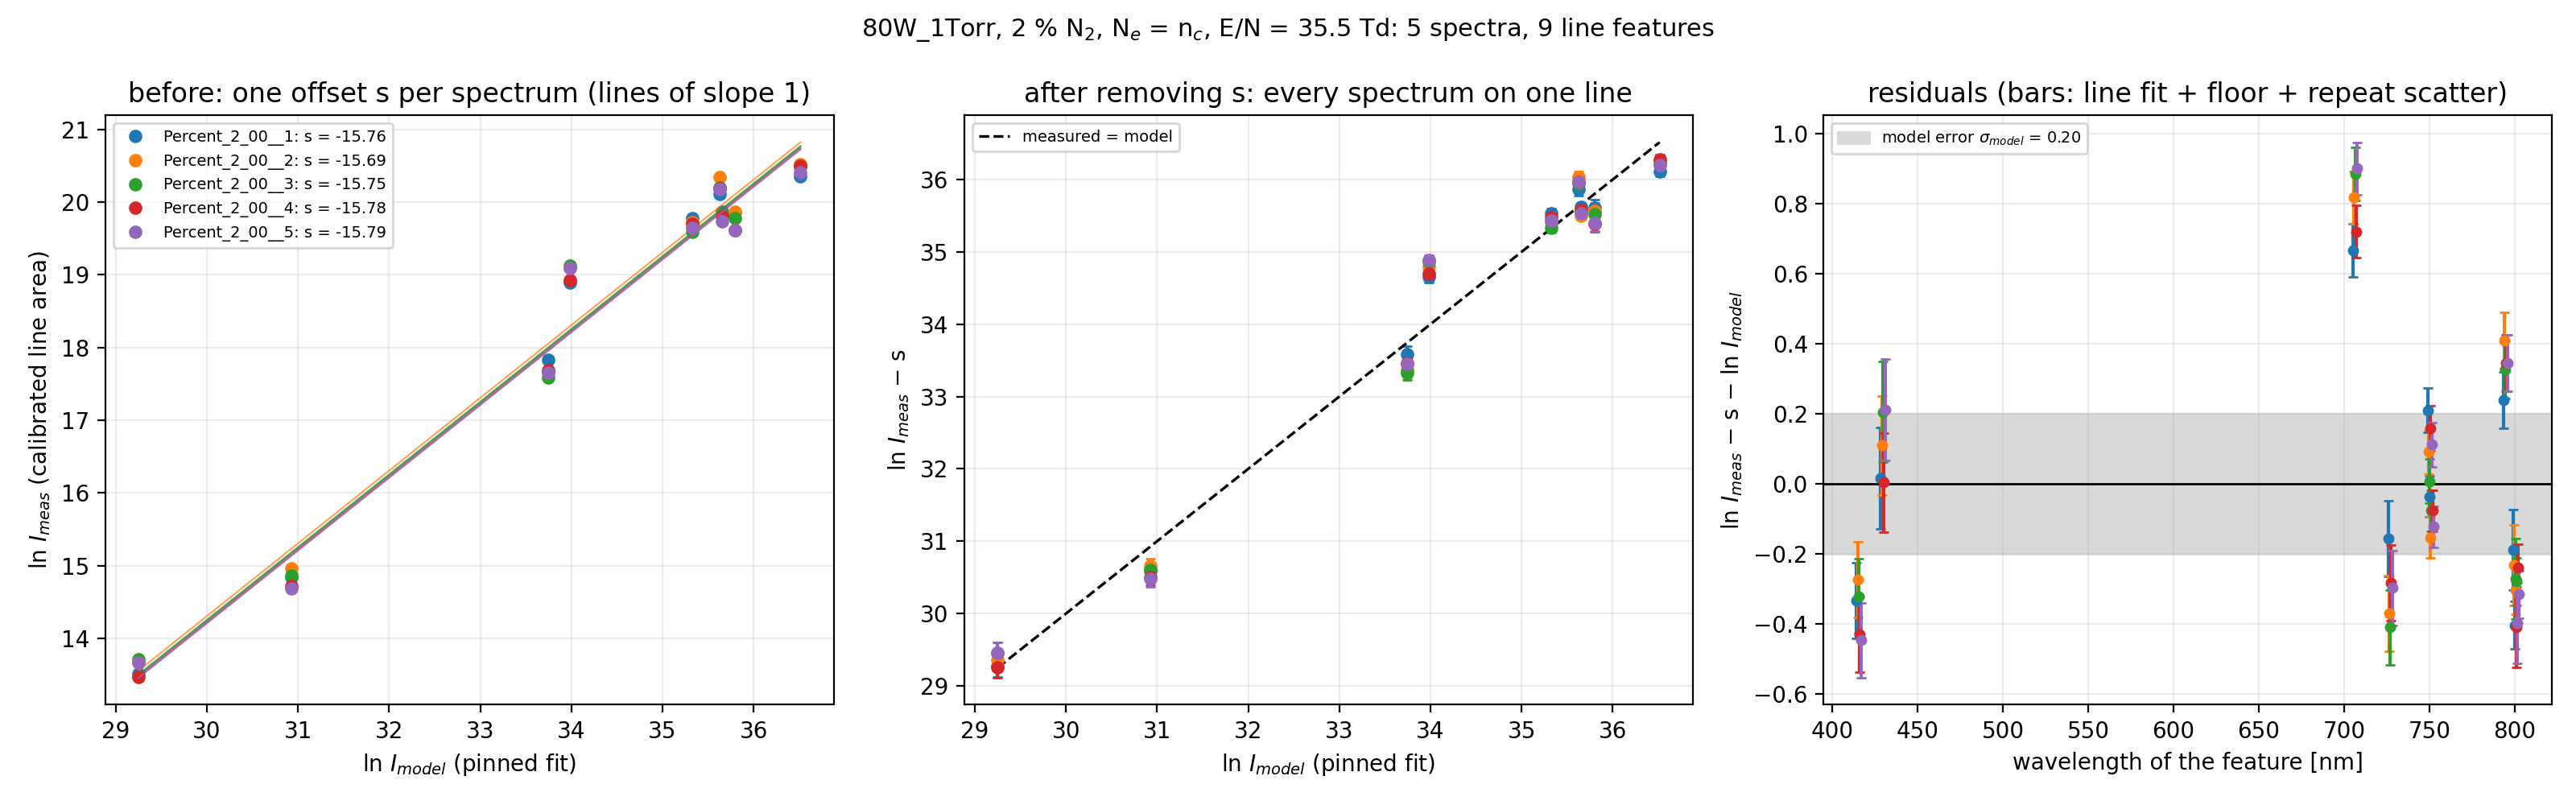
\includegraphics[width=\linewidth]{s_scale}
\caption{80\,W, 1\,Torr, 2\,\% N$_2$, at the fit with $N_e=\nc$. Left: measured against modelled feature intensities
of the five spectra, each with its own offset $s_a$. Middle: the same after subtracting $s_a$. Right: residuals per
feature; grey band: $\sigma_{\mathrm{model}}$.}
\label{fig:s}
\end{figure}

%======================================================================================================
\section{EEDF: which BOLSIG+ runs are made}
\label{sec:libraries}
%======================================================================================================
\paragraph{The EEDF family.} The EEDF is a two-term BOLSIG+ solution for \emph{pure argon} (Biagi cross sections)
in a 2.42\,GHz field, $\omega/N = 2\pi f/N$ with $N=p/(k_BT_g)$, on \NEN{} values of \EN{} from 3 to 1000\,Td (500
energy points; numerical precision $10^{-30}$ up to 150\,Td and $10^{-25}$ above, rows that time out or develop
run-away tails are redone at $10^{-25}$). The N$_2$ is left out of the Boltzmann equation but kept in the CR model
(quenching and dilution): the Ar/N$_2$ microwave EEDF does not fit these spectra (it needs $\sim$500\,Td and
overestimates the metastables $\sim$60 times), while the pure-Ar EEDF fits every N$_2$ fraction at $\nc$. The fit
parameter is \EN; it is reported together with $\Teff = \tfrac23\langle\varepsilon\rangle$ of the EEDF.

\paragraph{One library per $(p, T_g)$.} For each condition the gas temperature comes from a fit to all
2.40--2.45\,GHz LAS measurements (robust fit with a free offset per LAS run),
\begin{equation}
T_g = \TgZero\,\mathrm{K} + \TgAp\,\tfrac{\mathrm K}{\mathrm{Torr}}\,(p - 1\,\mathrm{Torr})
      + \TgAP\,\tfrac{\mathrm K}{\mathrm W}\,(P - 80\,\mathrm W) + \TgAx\,\tfrac{\mathrm K}{\%}\,x
      \TgAxxSign\,\TgAxx\,\tfrac{\mathrm K}{\%^2}\,x^2 ,
\end{equation}
($x$: \% N$_2$; scatter within a run $\approx\TgSigma$\,K), rounded to 50\,K (a data set may set $T_g$ instead).
The library depends only on $(p, T_g)$ --- pure Ar, the field frequency is fixed --- so every condition that rounds
to the same pair shares it: \NLib{} libraries for the \NCond{} conditions (Table~\ref{tab:libraries}). The CR table
also depends on the N$_2$ fraction (quenching and dilution): \NTab{} tables. Before fitting, the script lists the
missing libraries and tables (\texttt{--plan}) and builds them in parallel (a table takes 2--3\,min, six at a time);
existing ones are reused.

%======================================================================================================
\section{Choosing the best fit: $N_e$ free or pinned at $\nc$}
\label{sec:fit}
%======================================================================================================
$\chi^2$ of Eq.~\eqref{eq:chi2} is evaluated on a fine grid of 240 values of $\ln\EN$ $\times$ 220 values of
$\ln N_e$ (spline interpolation of the CR table).

\paragraph{Free fit.} The best fit is the global minimum $\chi^2_{\min}$ of the grid. The posterior is
\begin{equation}
p(\EN, N_e) \propto \exp\!\Big[-\frac{\chi^2 - \chi^2_{\min}}{2B^2}\Big],\qquad
B^2 = \max\!\Big(1, \frac{\chi^2_{\min}}{\nu}\Big),
\end{equation}
(log-uniform prior); the Birge factor $B$ widens it when the fit is worse than the errors allow. Medians and
16--84\,\% intervals are taken from its marginals. (Figure titles made by the analysis script write $B$ as ``s'';
it is unrelated to the per-spectrum scale $s_a$.)

\paragraph{Pinned fit.} The discharge is taken to be overdense, so the electron density near the surface where the
field is absorbed is the critical density
\begin{equation}
\nc = \frac{\varepsilon_0 m_e \omega^2}{e^2} = \Nc\ \mathrm{m}^{-3}\qquad (f = 2.42\ \mathrm{GHz}).
\end{equation}
The pinned fit uses the grid column nearest $\nc$: the best \EN{} is the minimum along it, and its band is
$\chi^2 \le \chi^2(\EN_{\mathrm{best}},\nc) + B^2$ along the column. $\Teff$ and the 1s densities are quoted at the
best \EN{} with their range over this band. $\chi^2$ per degree of freedom at $\nc$ is
$\chi^2(\EN_{\mathrm{best}},\nc)/(\nu+1)$ (one parameter fewer), and the \emph{cost of the pin} is
$[\chi^2(\EN_{\mathrm{best}},\nc)-\chi^2_{\min}]/B^2$. The actinometry uses the posterior restricted to the same
column (renormalised).

\paragraph{What the $\chi^2$ surface looks like.} Figure~\ref{fig:freevsnc} shows two valleys: a cold, dense
branch (\EN{} $\approx 8$--10\,Td running to the $N_e$ grid edge at $3\times10^{19}$\,m$^{-3}$, where stepwise
excitation through the 4s levels makes up for the weak EEDF tail) and a branch near $10^{17}$\,m$^{-3}$ at
\EN{} $\approx 35$\,Td that passes through $\nc$. Along each valley more electrons trade against a cooler EEDF, so
the lines alone constrain $N_e$ only weakly. At 0.33\,\% N$_2$ the global minimum is on the dense branch and the pin
costs $6.8\,B^2$; at 2\,\% the free minimum is at $1.5\times10^{17}$\,m$^{-3}$, twice $\nc$, and the pin costs
$1.0\,B^2$.

\begin{figure}[H]
\centering
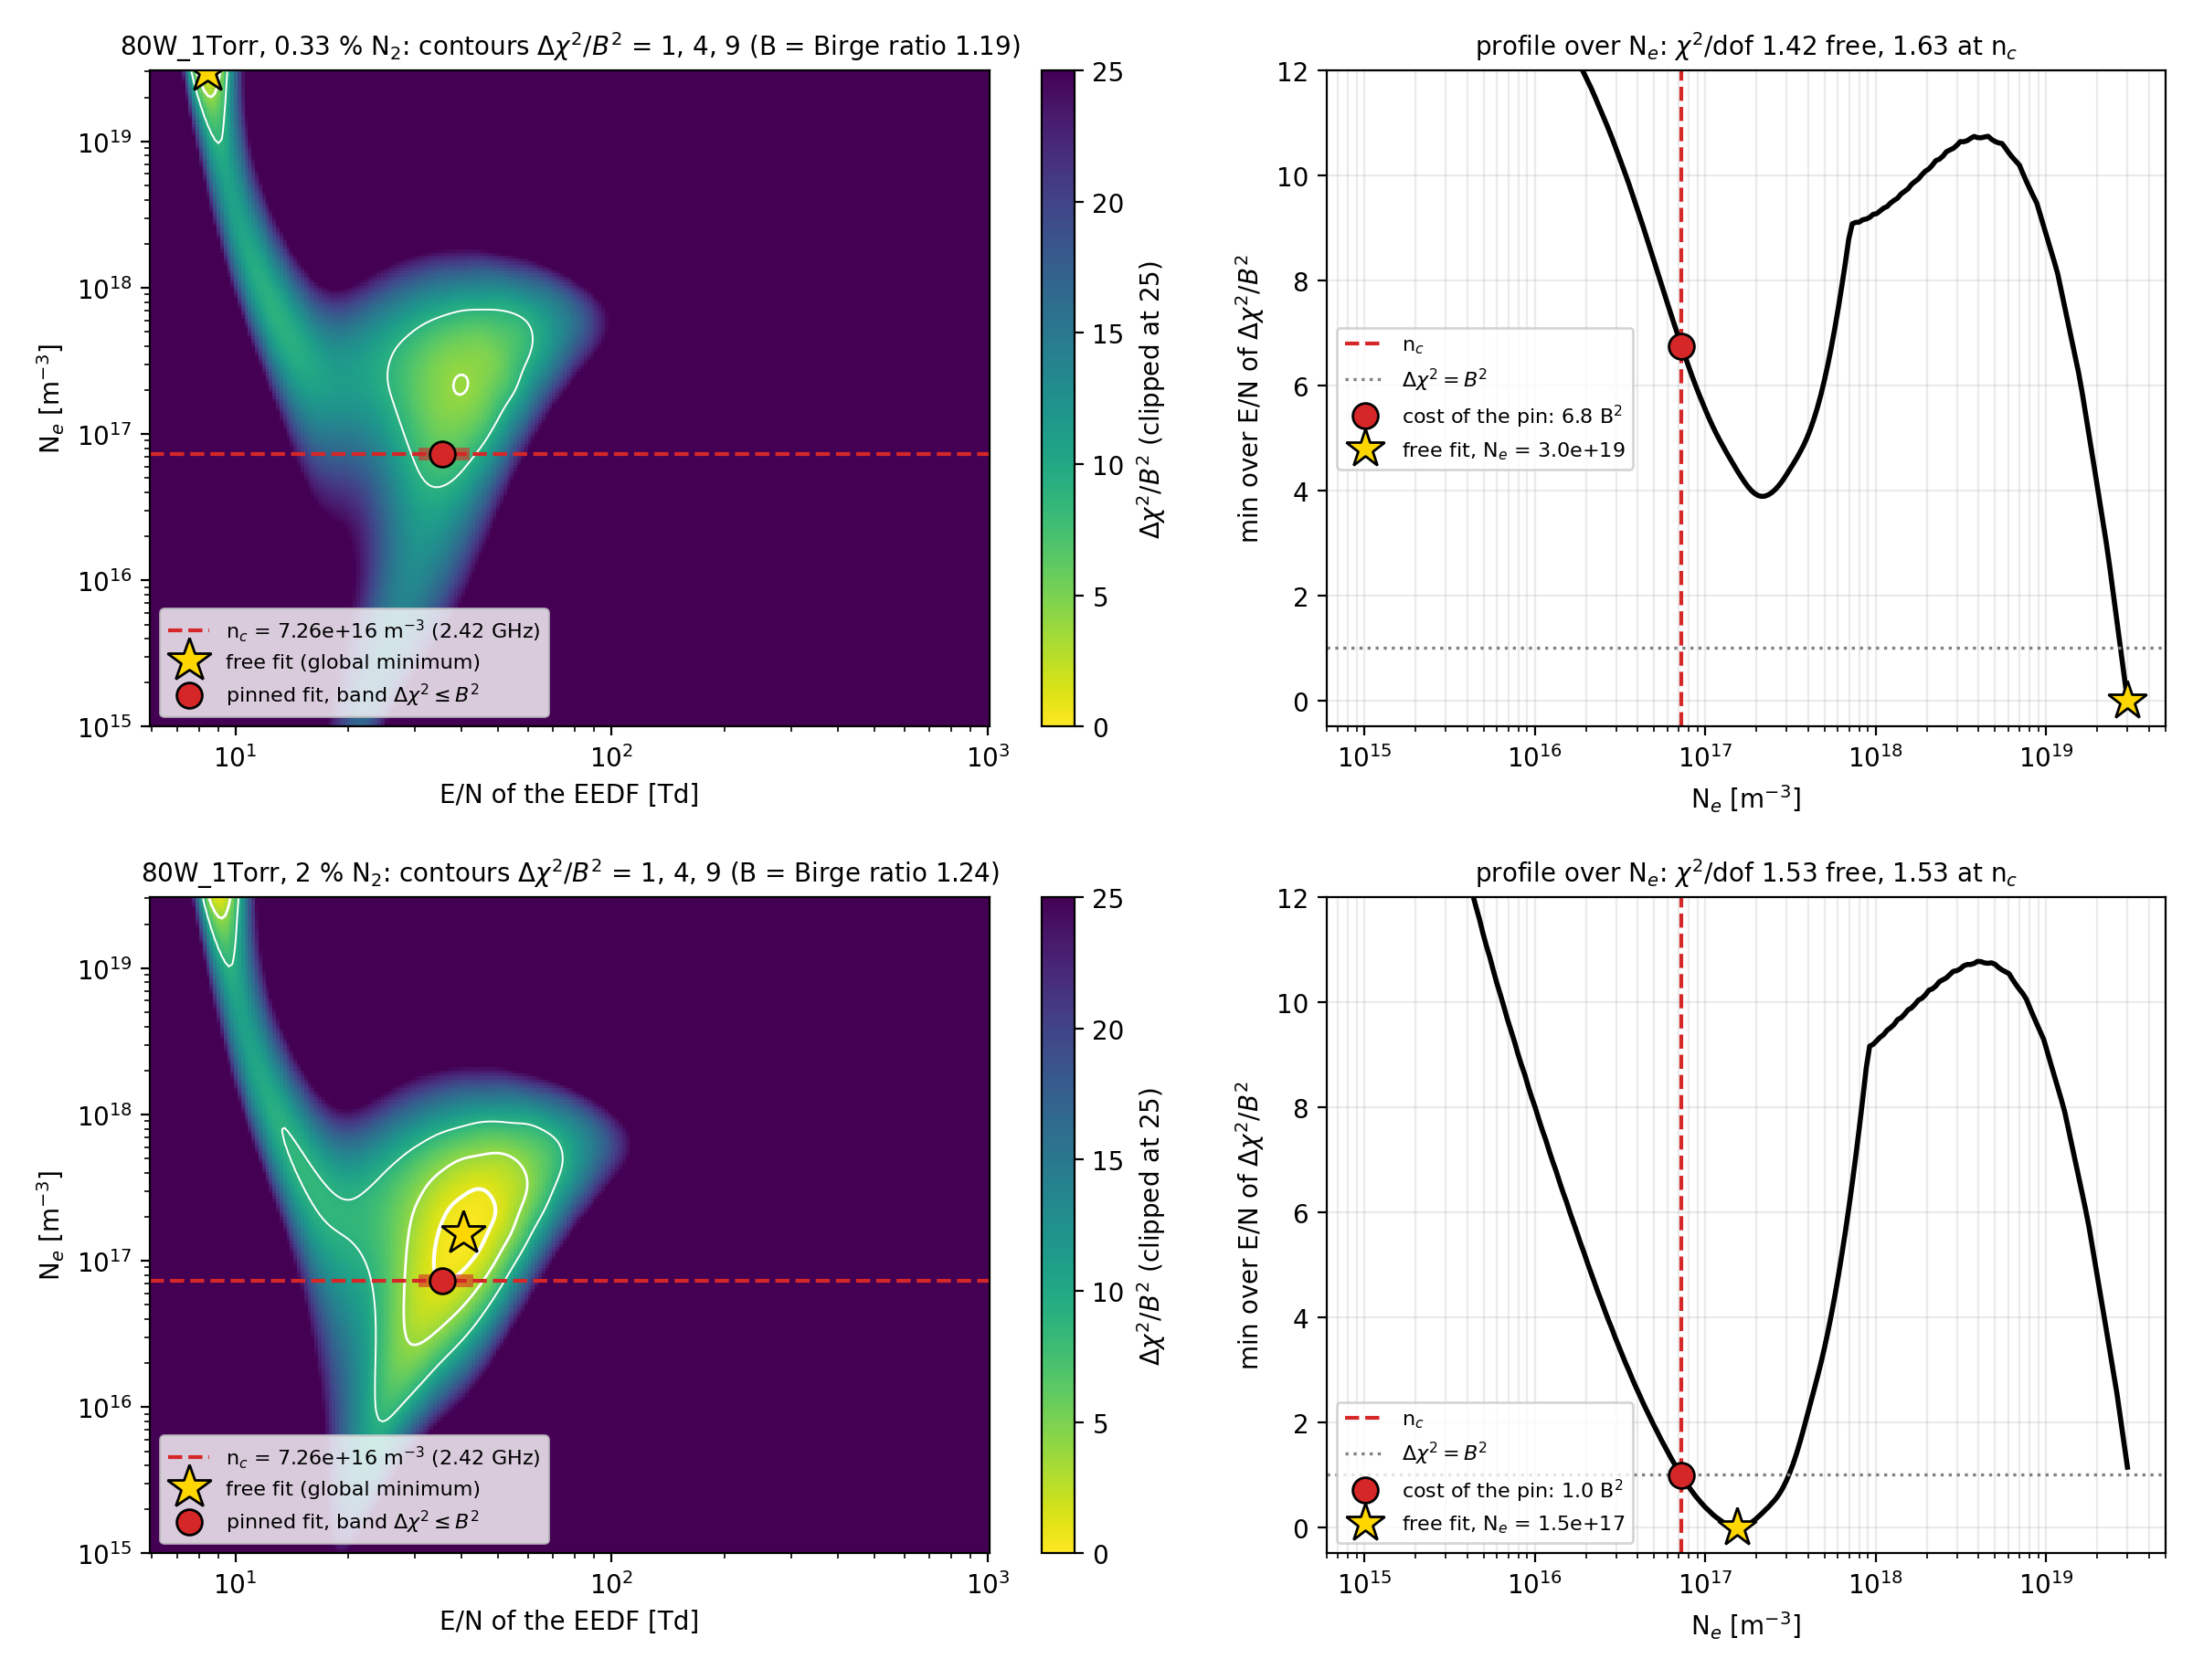
\includegraphics[width=0.94\linewidth]{fit_free_vs_nc}
\caption{$\Delta\chi^2/B^2$ over $(\EN, N_e)$ (left) and its minimum over \EN{} for each $N_e$ (right) for 80\,W,
1\,Torr at 0.33 and 2\,\% N$_2$. Star: free fit; red circle and bar: fit at $\nc$ and its band.}
\label{fig:freevsnc}
\end{figure}

Over all conditions (Fig.~\ref{fig:pincost}, Table~\ref{tab:fits}): in the N$_2$ sweeps the free fit runs to the grid edge from 0 to about 1--1.3\,\% N$_2$, where the pin costs
3--11\,$B^2$; above that the free minimum sits at $(1$--$2.2)\times10^{17}$\,m$^{-3}$ (one exception: 60\,W
at 1.66\,\%, at the edge) and the pin costs at most $2.3\,B^2$. In the 3\,\% pressure sweep the free $N_e$ is
$(0.9$--$2.8)\times10^{17}$\,m$^{-3}$ everywhere; the pin costs 3.5--7\,$B^2$ at 600--800\,mTorr, at most
$2.9\,B^2$ from 850\,mTorr and less than $1.5\,B^2$ above 1000\,mTorr. $\chi^2$ per degree of freedom is 1.2--3.0 at $\nc$ (typically 1.4--1.9) and
barely lower when $N_e$ is free. All results below are at $\nc$.

\begin{figure}[H]
\centering
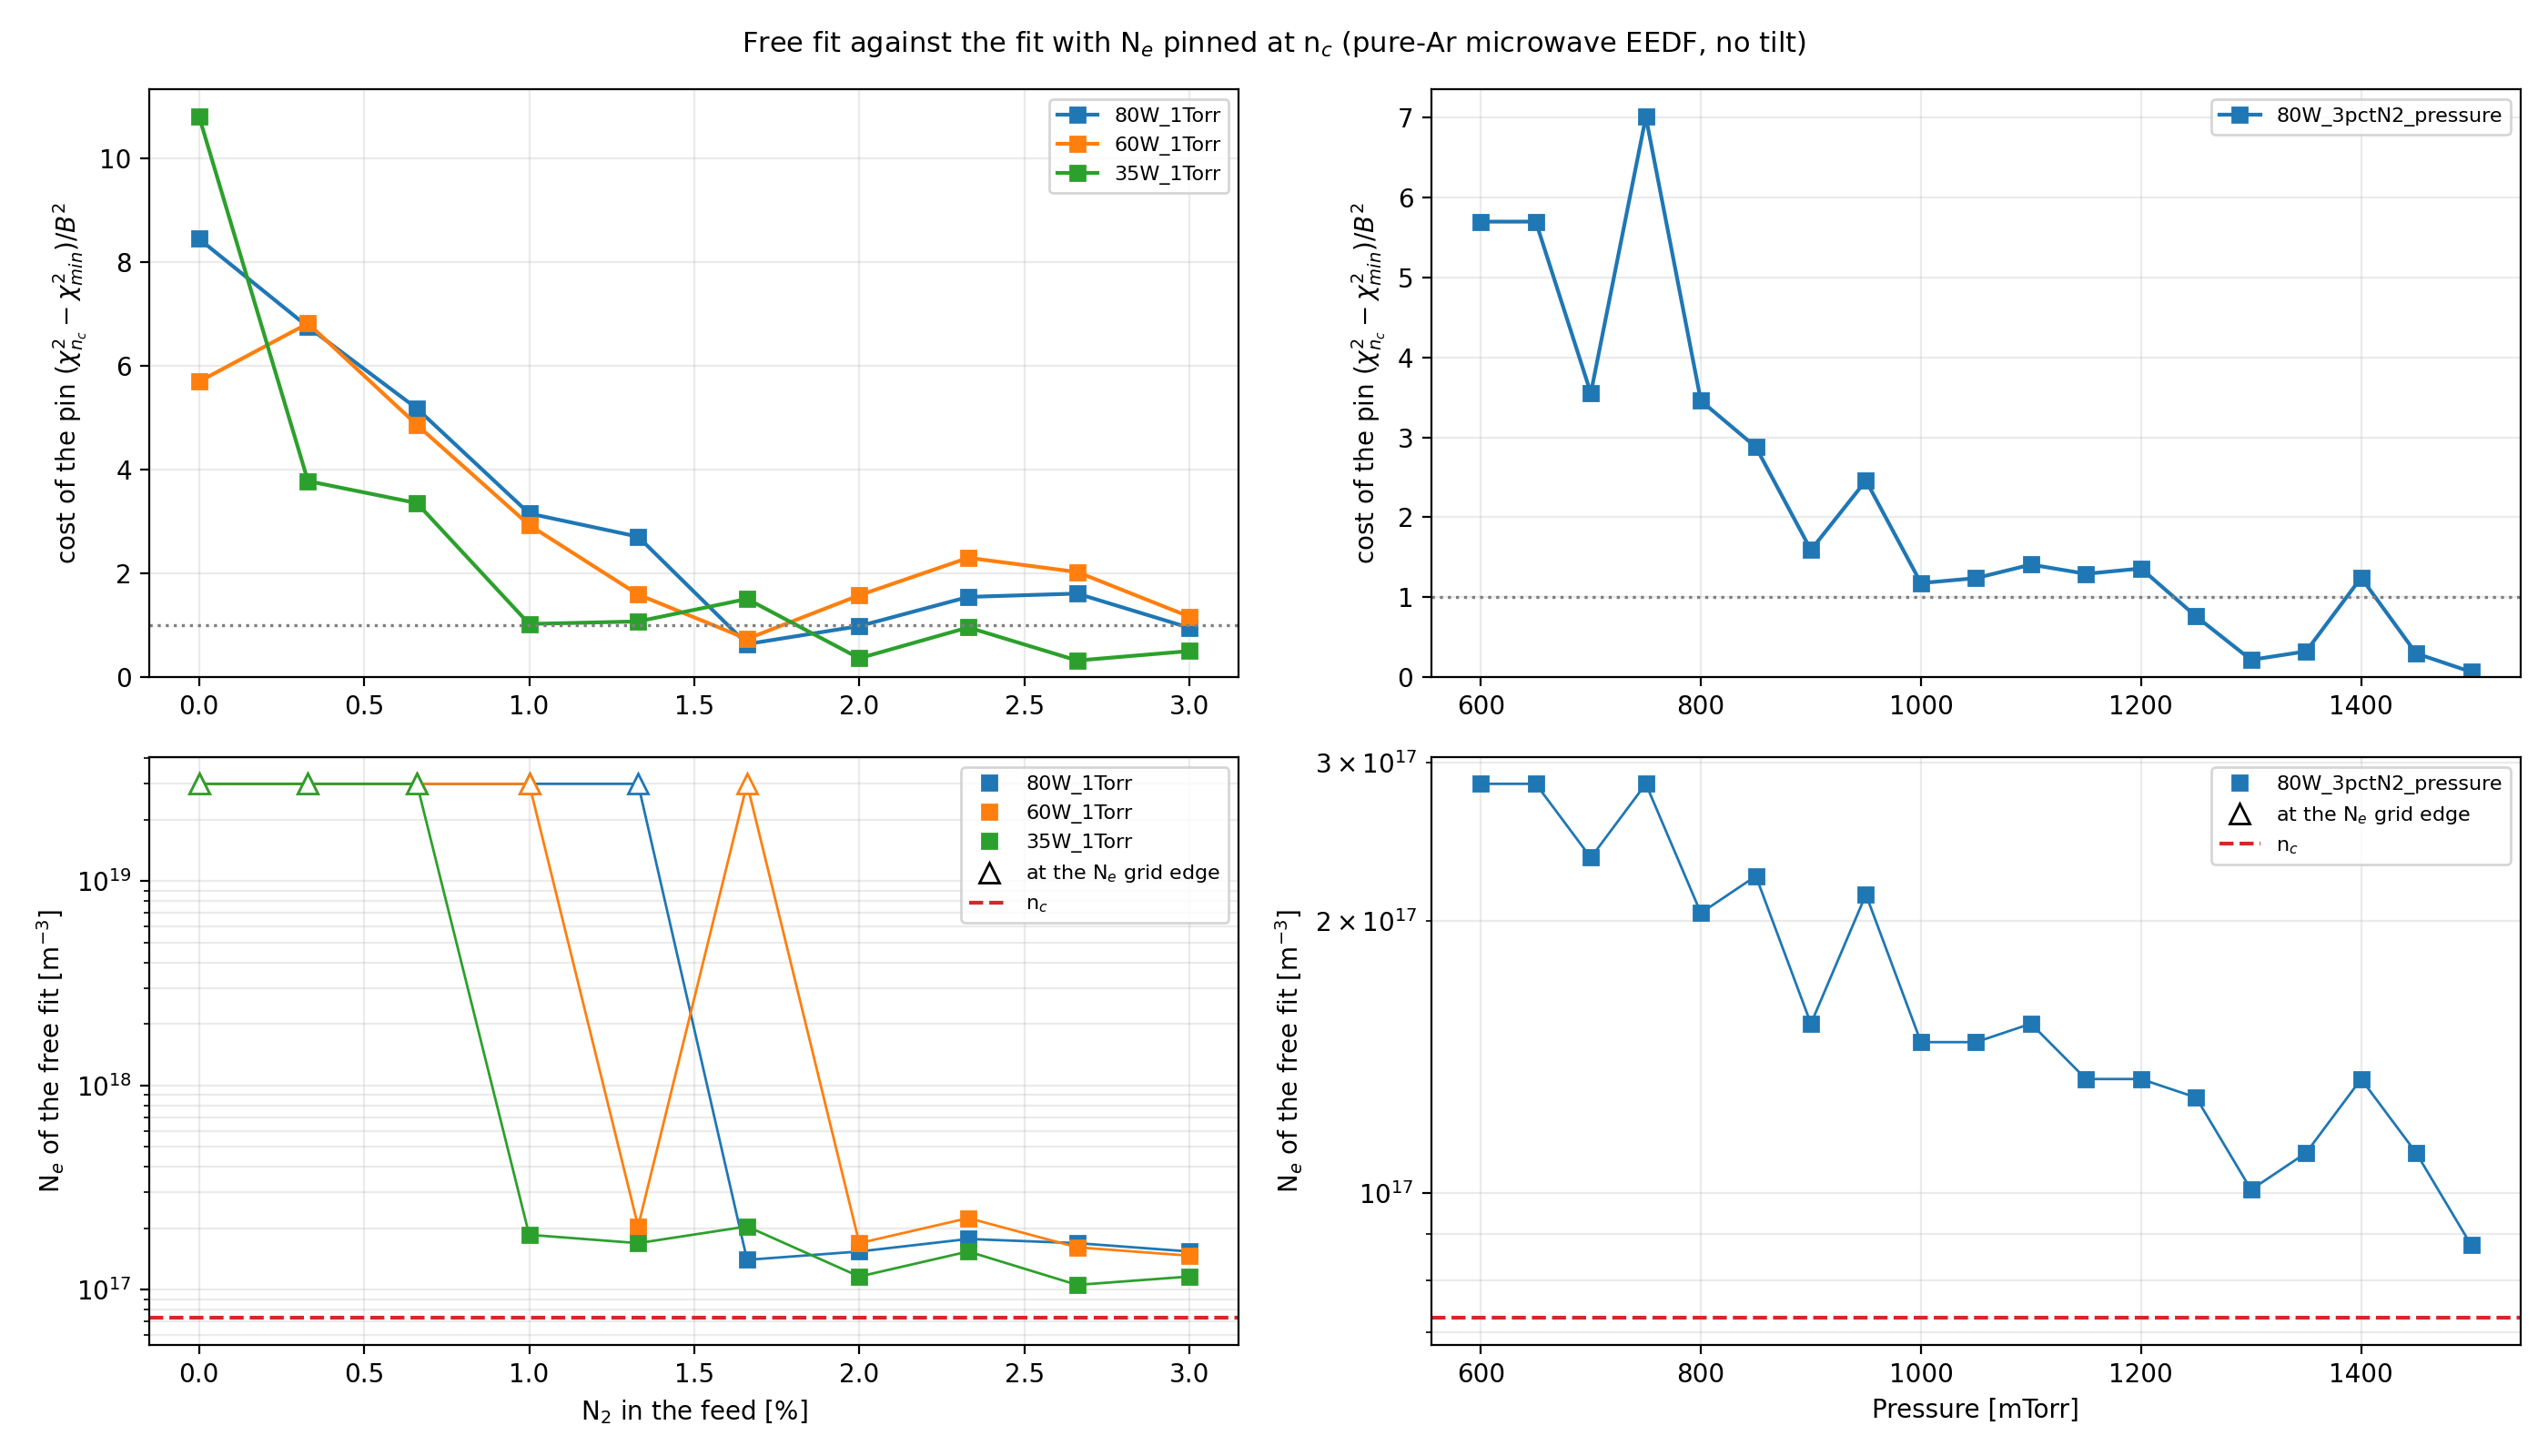
\includegraphics[width=0.9\linewidth]{pin_cost}
\caption{Cost of pinning $N_e$ at $\nc$ (top) and $N_e$ of the free fit (bottom; open triangles: at the grid edge)
for the N$_2$ sweeps (left) and the pressure sweep (right).}
\label{fig:pincost}
\end{figure}

%======================================================================================================
\section{Fit results: E/N, $T_{e,\mathrm{eff}}$ and the Ar metastables}
\label{sec:results}
%======================================================================================================
At $\nc$ the N$_2$ sweeps give \EN{} = 32--44\,Td at every N$_2$ fraction and power (Fig.~\ref{fig:enN2}); $\Teff$
stays at 0.81--0.82\,eV, since the mean energy of the microwave EEDF hardly changes in this \EN{} range. In the
3\,\% pressure sweep \EN{} falls from 62\,Td at 600\,mTorr to 31\,Td at 1500\,mTorr (Fig.~\ref{fig:psweep}).

The CR 1s$_5$ density at the fit agrees with LAS within 10--16\,\% in pure Ar but falls faster with N$_2$: CR/LAS is
0.36 (80\,W), 0.50 (60\,W) and 0.74 (35\,W) at 3\,\% N$_2$ (Fig.~\ref{fig:metaN2}). In the pressure sweep CR/LAS
rises from 0.23 at 600\,mTorr to 0.59 at 1500\,mTorr. The model's N$_2$ quenching of the 4s levels (or a missing
production channel) is the first suspect.

\begin{figure}[H]
\centering
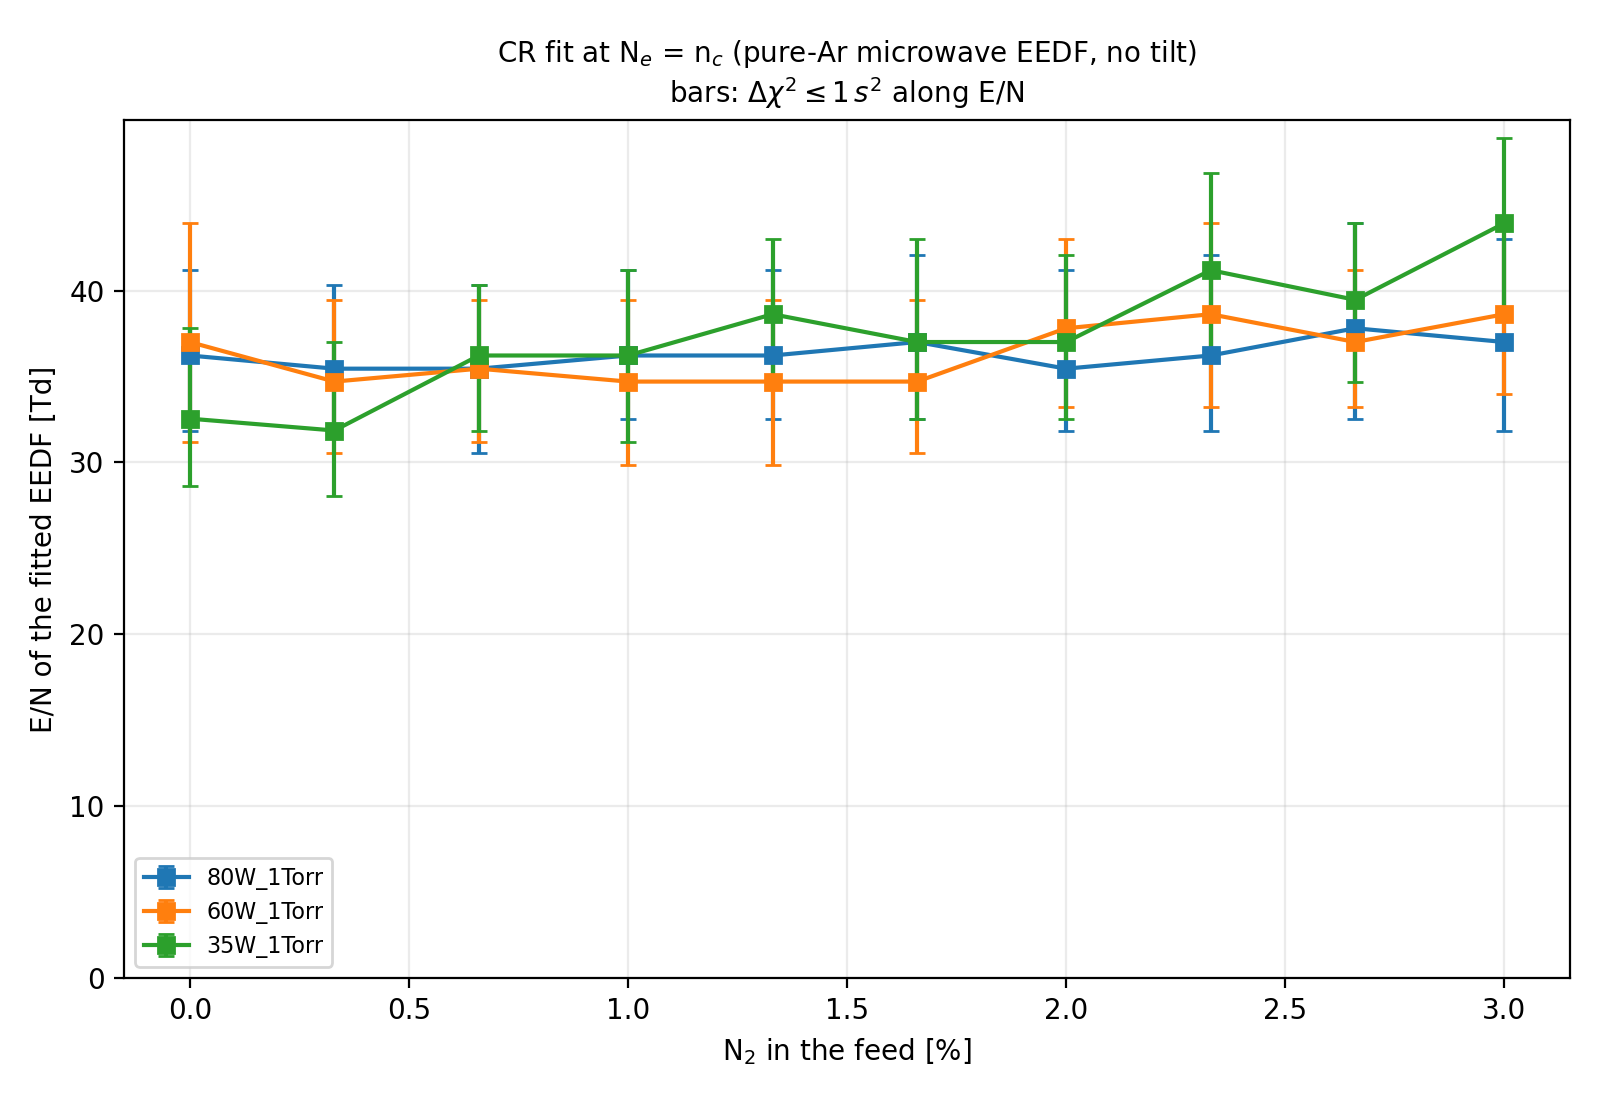
\includegraphics[width=0.49\linewidth]{ov_N2_EN}\hfill
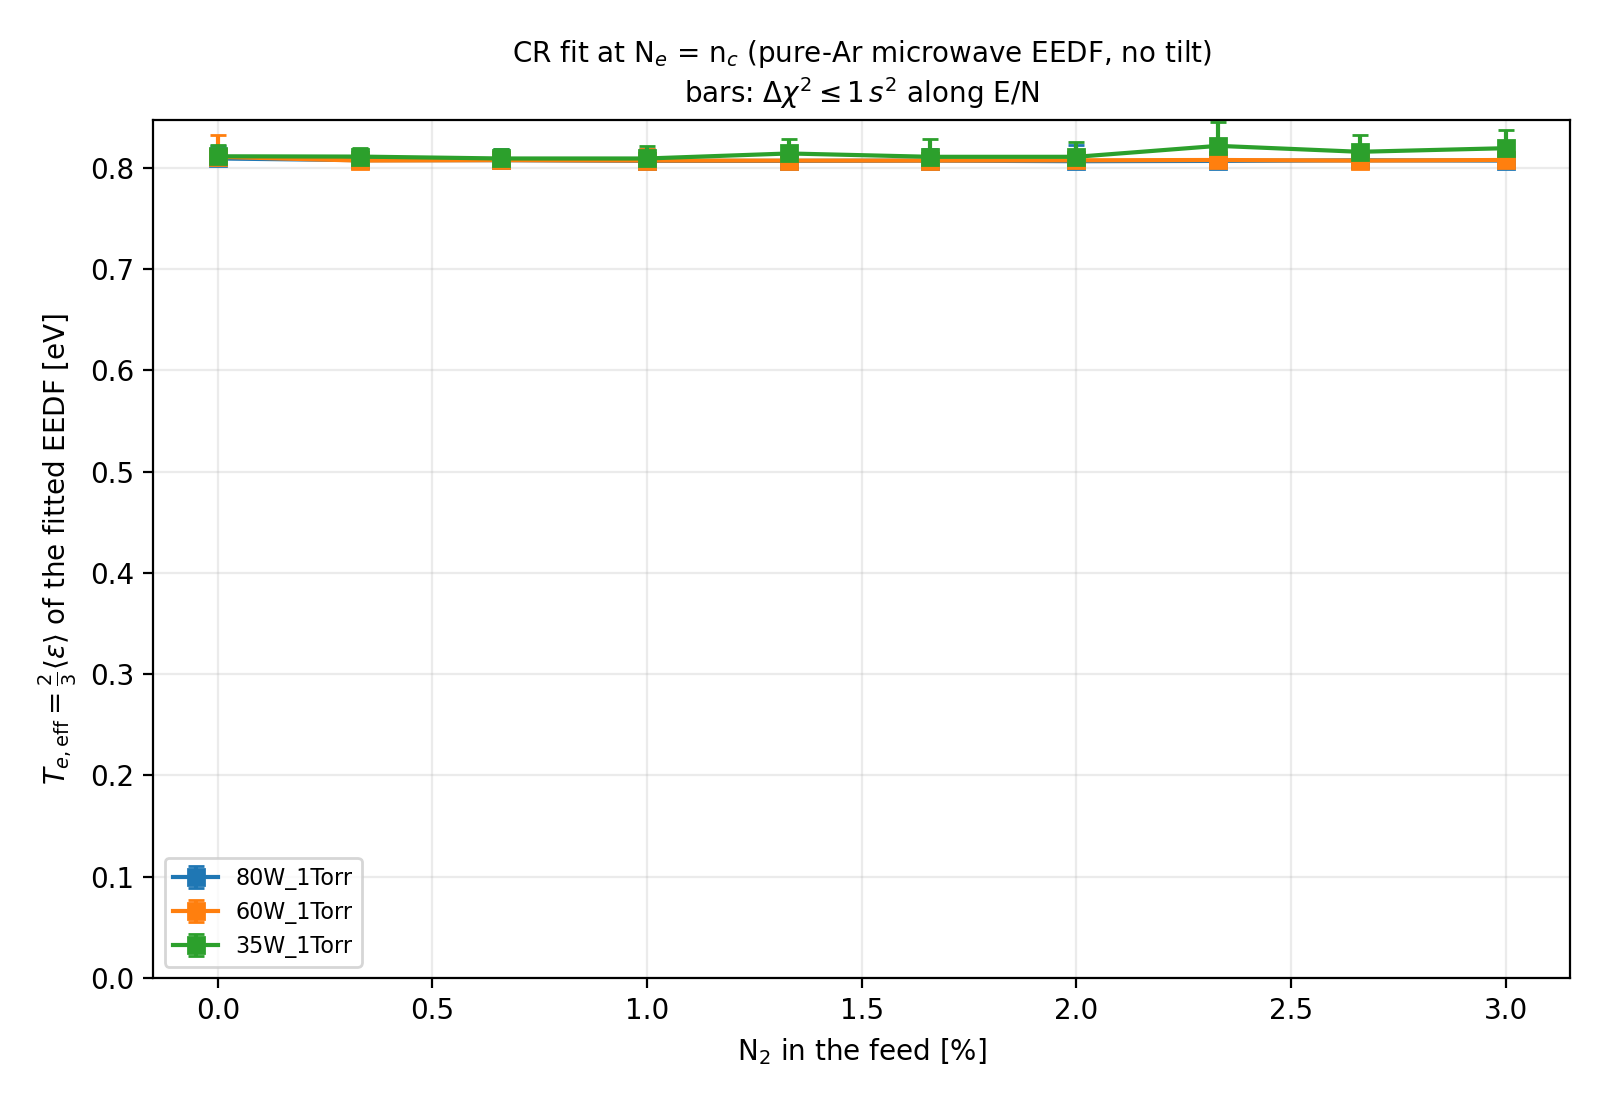
\includegraphics[width=0.49\linewidth]{ov_N2_Te_eff}
\caption{\EN{} (left) and $\Teff$ (right) of the fit at $\nc$ for the three N$_2$ sweeps; bars: $\Delta\chi^2\le B^2$
along \EN.}
\label{fig:enN2}
\end{figure}

\begin{figure}[H]
\centering
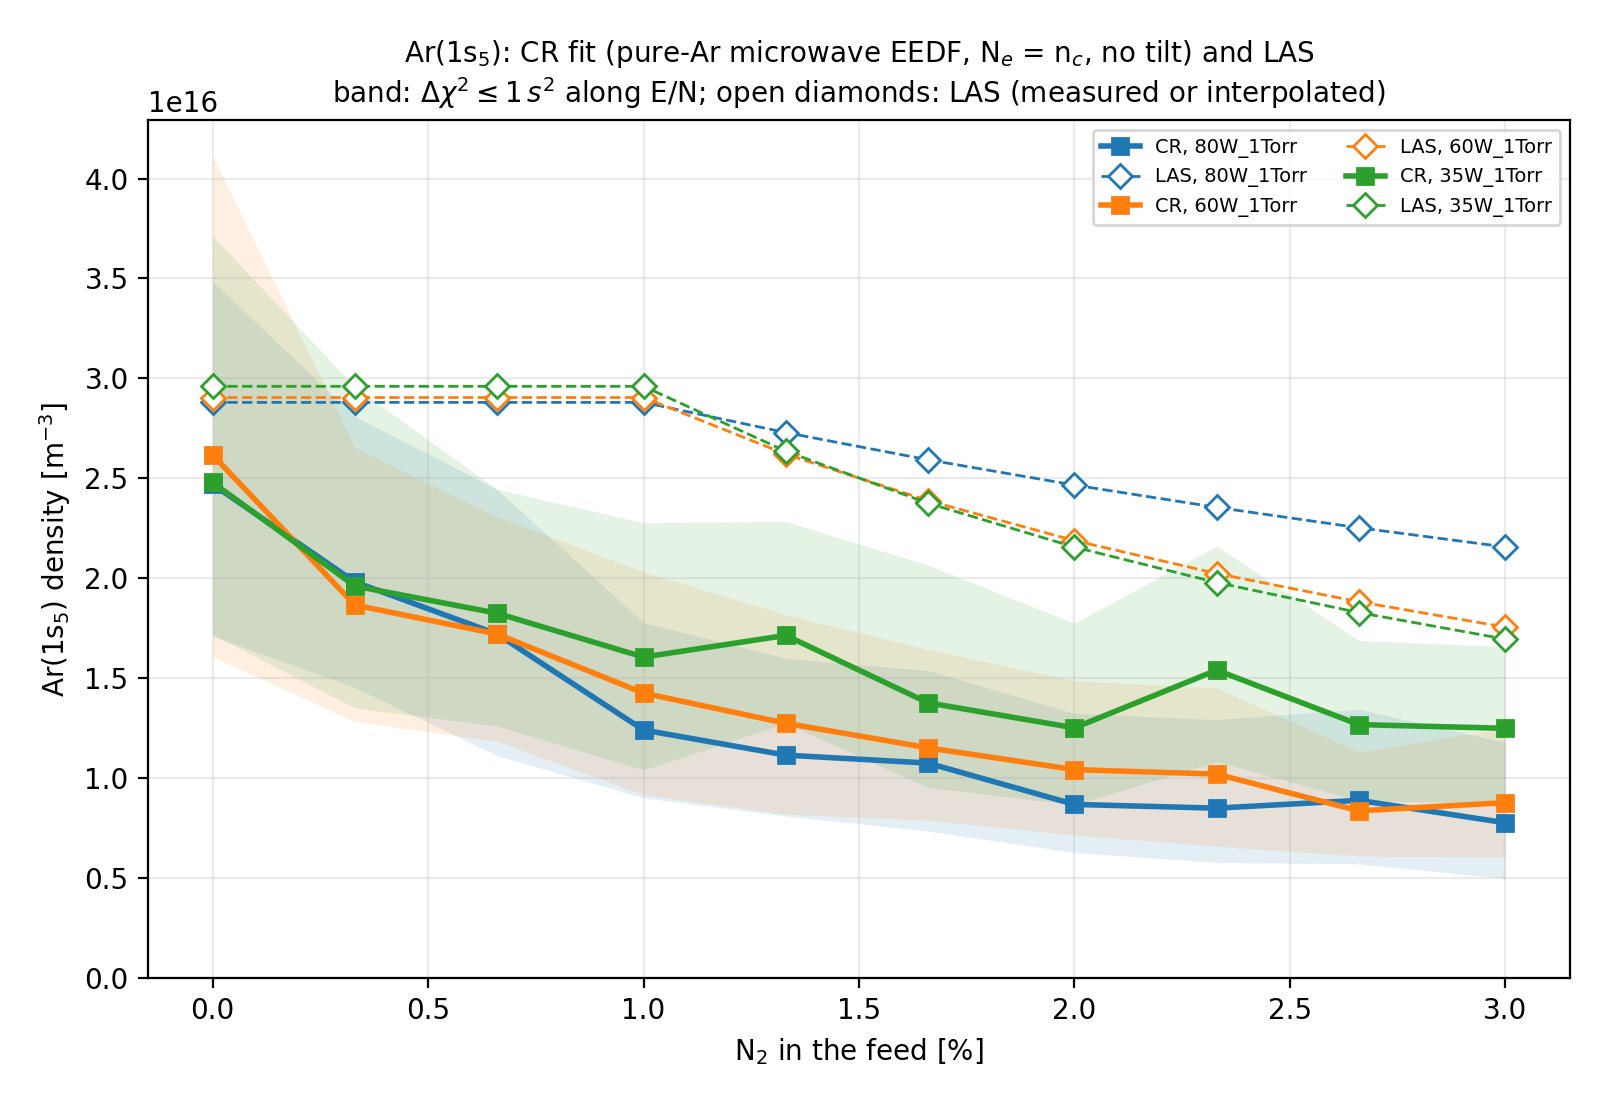
\includegraphics[width=0.62\linewidth]{ov_N2_1s5}
\caption{Ar(1s$_5$): CR model at the fit (filled, band $\Delta\chi^2\le B^2$) and LAS (open diamonds, measured or
interpolated to the condition) for the N$_2$ sweeps.}
\label{fig:metaN2}
\end{figure}

\begin{figure}[H]
\centering
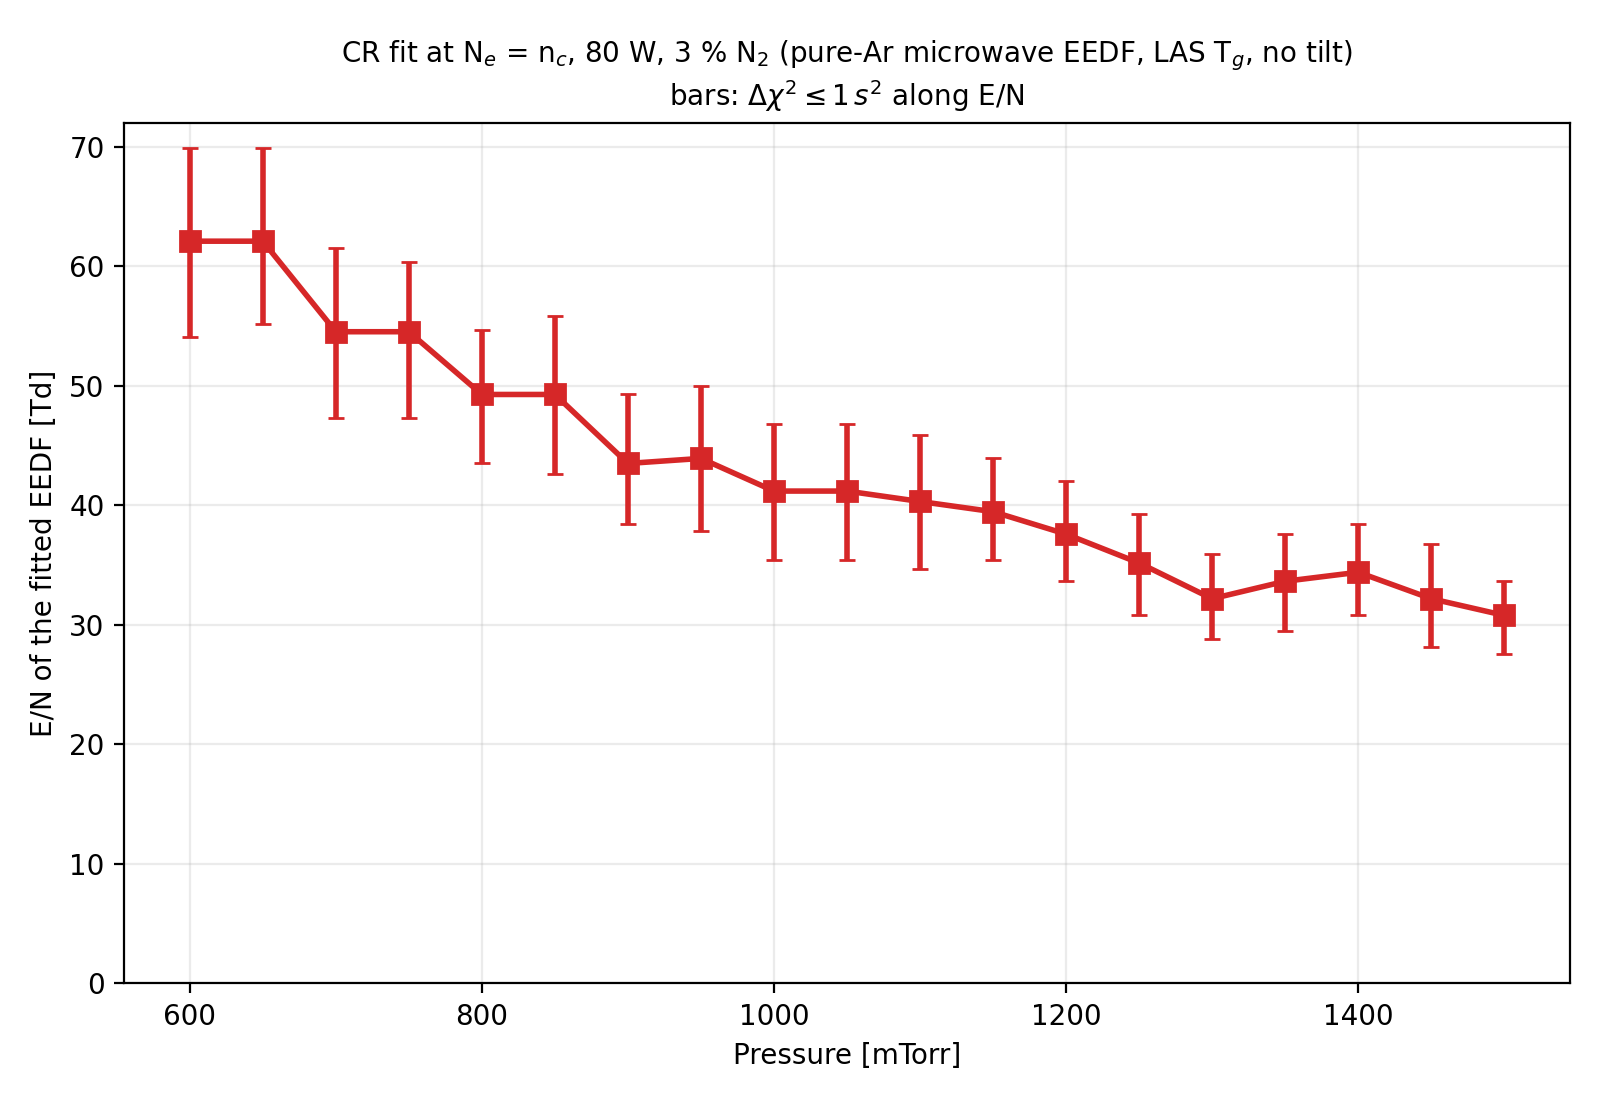
\includegraphics[width=0.49\linewidth]{p_EN}\hfill
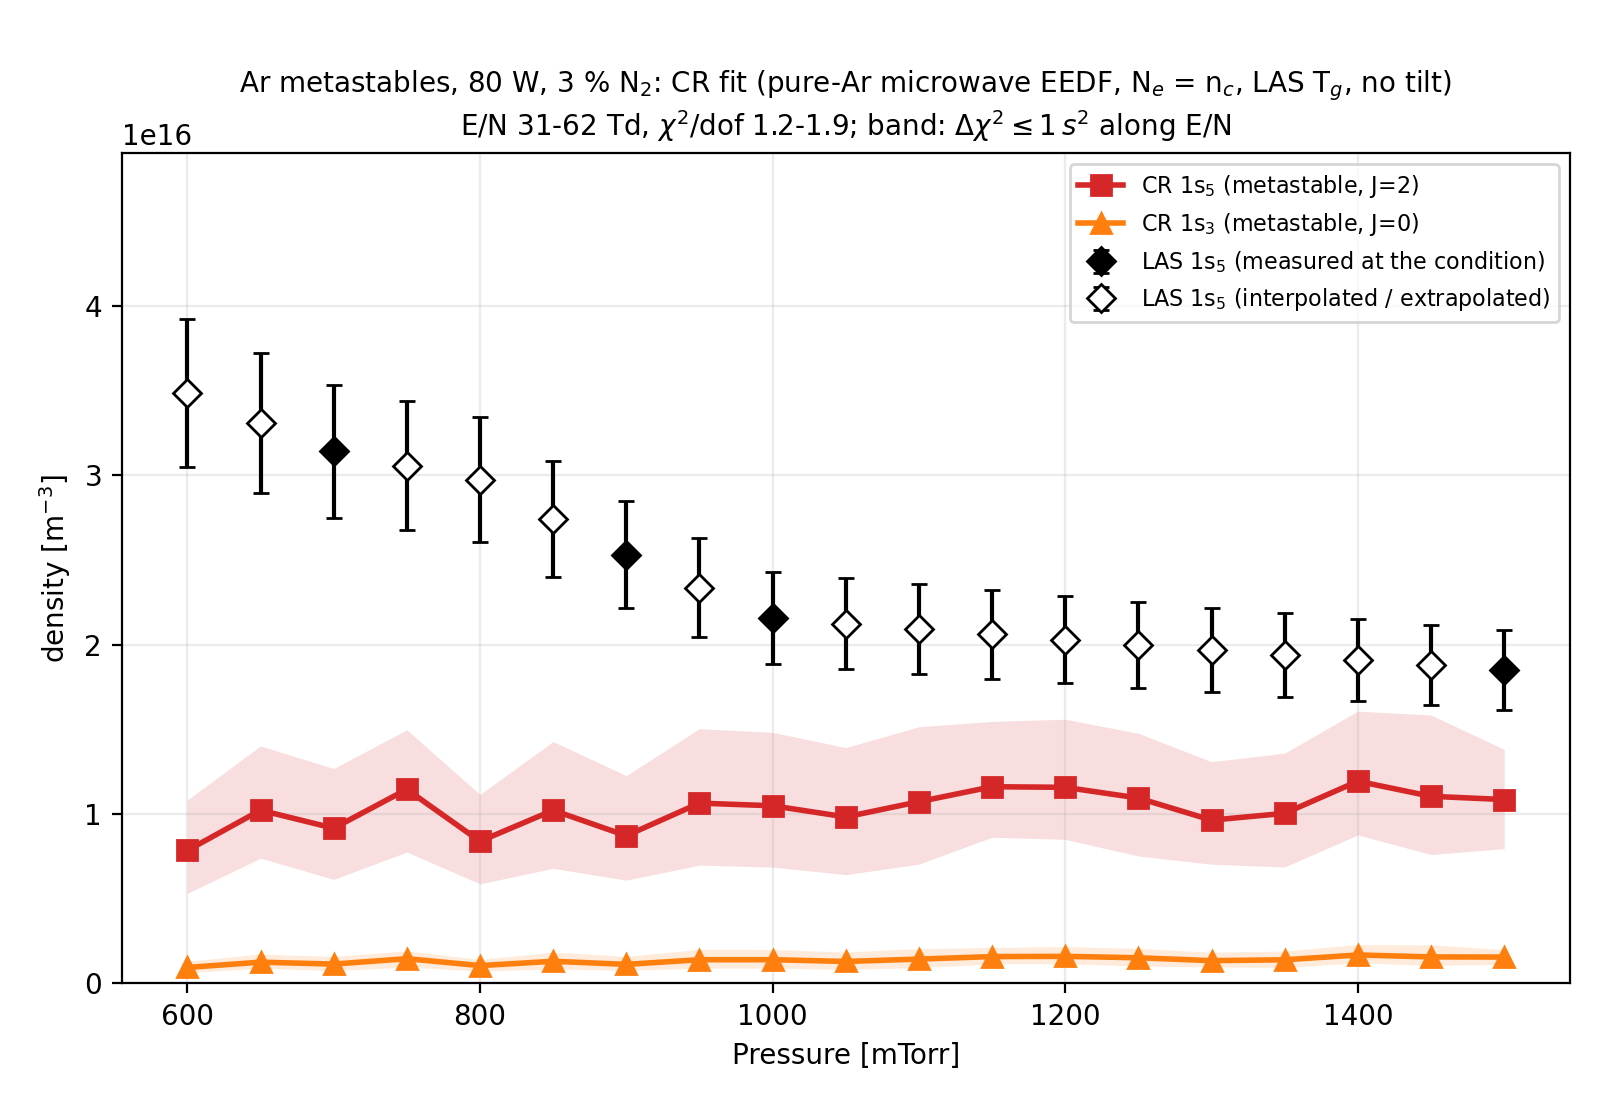
\includegraphics[width=0.49\linewidth]{p_metastables}
\caption{Pressure sweep (80\,W, 3\,\% N$_2$): \EN{} at $\nc$ (left) and the CR 1s$_5$/1s$_3$ densities against LAS
(right).}
\label{fig:psweep}
\end{figure}

%======================================================================================================
\section{Actinometry: atomic nitrogen}
\label{sec:actinometry}
%======================================================================================================
\paragraph{Lines.} N\,I 744.23 and 746.83\,nm, both from 3p\,$^4$S$^\circ_{3/2}$ (A = $1.19\times10^7$ and
$1.96\times10^7$\,s$^{-1}$, branching ratios 0.320 and 0.528; the third line, 742.36\,nm, falls in an echelle gap).
746.83\,nm is stronger (SNR 4--6 against $\sim$2.5) and detected in 67--87\,\% of the spectra against 42--59\,\%, so
every N$_2$ condition has a result. Since both come from the same level, their measured ratio must equal the ratio of
$A/\lambda$ (1.64); deviations reveal calibration problems, blends or N$_2$ bands (Fig.~\ref{fig:sameupper}). The
Ar\,I references are the 4p and 5p lines of the line selection without 706.72, 415.86 and 794.82\,nm, which lie off
the other pairs by 1.5--2.5$\times$ at every condition.

\paragraph{Formula.} For an N\,I / Ar\,I pair with measured (calibrated, energy-unit) line ratio $I_N/I_{Ar}$,
\begin{align}
\text{without metastables:}\quad
\frac{n_N}{n_{Ar}} &= \frac{I_N}{I_{Ar}}\,\frac{\lambda_N}{\lambda_{Ar}}\,
  \frac{k_{Ar}\,b_{Ar}}{k_N\,b_N}, \\
\text{with metastables (CR):}\quad
\frac{n_N}{n_{Ar}} &= \frac{I_N}{I_{Ar}}\,\frac{\lambda_N}{\lambda_{Ar}}\,
  \frac{I^{\mathrm{CR}}_{Ar}/(N_e\, n_{Ar})}{k_N\,b_N},
\end{align}
where $k$ are the ground-state excitation rate coefficients of the upper levels (BSR N\,I cross section for
3p\,$^4$S$^\circ$; for Ar the CR model's own cross sections) integrated over the fitted EEDF, $b$ the branching
ratios and $\lambda_N/\lambda_{Ar}$ converts energy to photon units. In the CR variant the Ar reference line is
described by the CR model's emission of that line per Ar atom and electron, $I^{\mathrm{CR}}_{Ar}/(N_e n_{Ar}) =
n_u A\eta/(N_e n_{Ar})$, which includes stepwise excitation from the metastable and resonant 4s levels, cascades,
collisional losses of the upper level and trapping. The N\,I level is assumed to be excited from ground-state N
atoms only (no dissociative excitation of N$_2$, no stepwise excitation through N($^2$D, $^2$P)).

\paragraph{From pairs to one number.} For every pair the expression is evaluated on the \EN{} axis at $\nc$ and
pushed through the pinned posterior (median and 16--84\,\%); a pair needs 90\,\% of the posterior mass in the range
where both rate coefficients are valid (EEDF reaching threshold + 1\,eV). Per condition (with at least five valid
pairs) pairs whose median lies outside the Tukey fences $[Q_1 - 1.5\,\mathrm{IQR}, Q_3 + 1.5\,\mathrm{IQR}]$ of
$\ln(n_N/n_{Ar})$ are outliers and left out. The rest are averaged at every \EN{} point with weights
$1/\sigma^2$ of their line ratios before the posterior quantiles are taken, so the \EN{} uncertainty they share is
not averaged down. The error of $\ln(n_N/n_{Ar})$ is
\begin{equation}
\sigma_{\mathrm{stat}}^2 = \sigma_{\EN}^2 + \sigma_{\mathrm{meas}}^2,\qquad
\sigma_{\mathrm{meas}} = \frac{\max(1, B_{\mathrm{pairs}})}{\sqrt{\sum w}},\qquad
\sigma_{\mathrm{total}}^2 = \sigma_{\mathrm{stat}}^2 + 0.20^2 + 0.15^2 ,
\end{equation}
with $\sigma_{\EN}$ half the 16--84\,\% width, $B_{\mathrm{pairs}}$ the Birge ratio of the pairs and the cross-section
errors of N (20\,\%) and Ar (15\,\%) as a systematic common to all conditions. With the feed fraction $f$ of N$_2$,
\begin{equation}
n_N = \frac{n_N}{n_{Ar}}\,(1-f)\,\frac{p}{k_BT_g},\qquad
\text{dissociation degree} = \frac{n_N}{2 n_{N_2}} = \frac{n_N}{n_{Ar}}\,\frac{1-f}{2f},
\end{equation}
the latter assuming that little N$_2$ is dissociated ($n_{N_2}/n_{Ar}\approx f/(1-f)$).

\paragraph{Results.} With metastables the pairs agree (Birge ratio 1.1--1.2, median $\sigma_{\mathrm{stat}}$
0.10--0.14 in $\ln$): $n_N/n_{Ar} = (1.3$--$8.1)\times10^{-4}$ in the N$_2$ sweeps and $(4.0$--$9.6)\times10^{-4}$ in
the pressure sweep, $n_N = 2\times10^{18}$--$1.6\times10^{19}$\,m$^{-3}$, dissociation 0.7--3.7\,\%
(Figs.~\ref{fig:actN2}, \ref{fig:actp}, Table~\ref{tab:actinometry}). Without metastables the values are 3--6 times
lower and the pairs disagree (Birge ratio 2--3.5): ground-state excitation alone does not describe the Ar reference
lines at $\nc$ (Fig.~\ref{fig:variants}).

\begin{figure}[H]
\centering
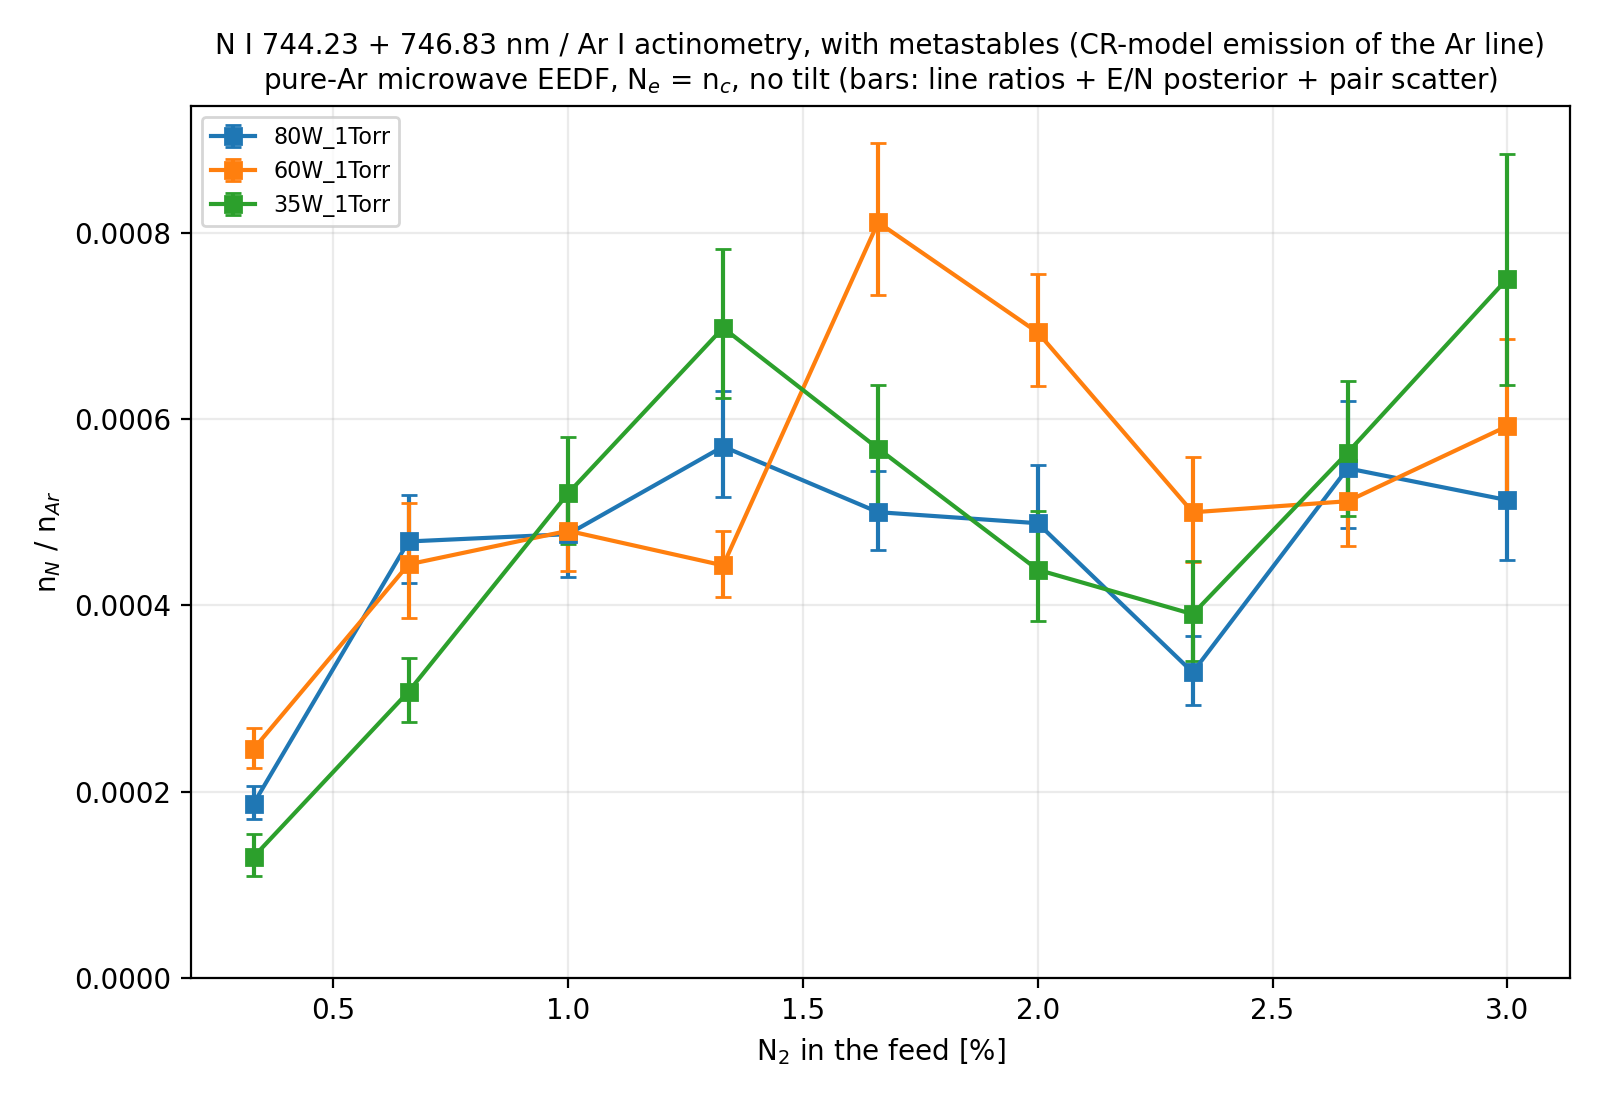
\includegraphics[width=0.49\linewidth]{ov_N2_actinometry}\hfill
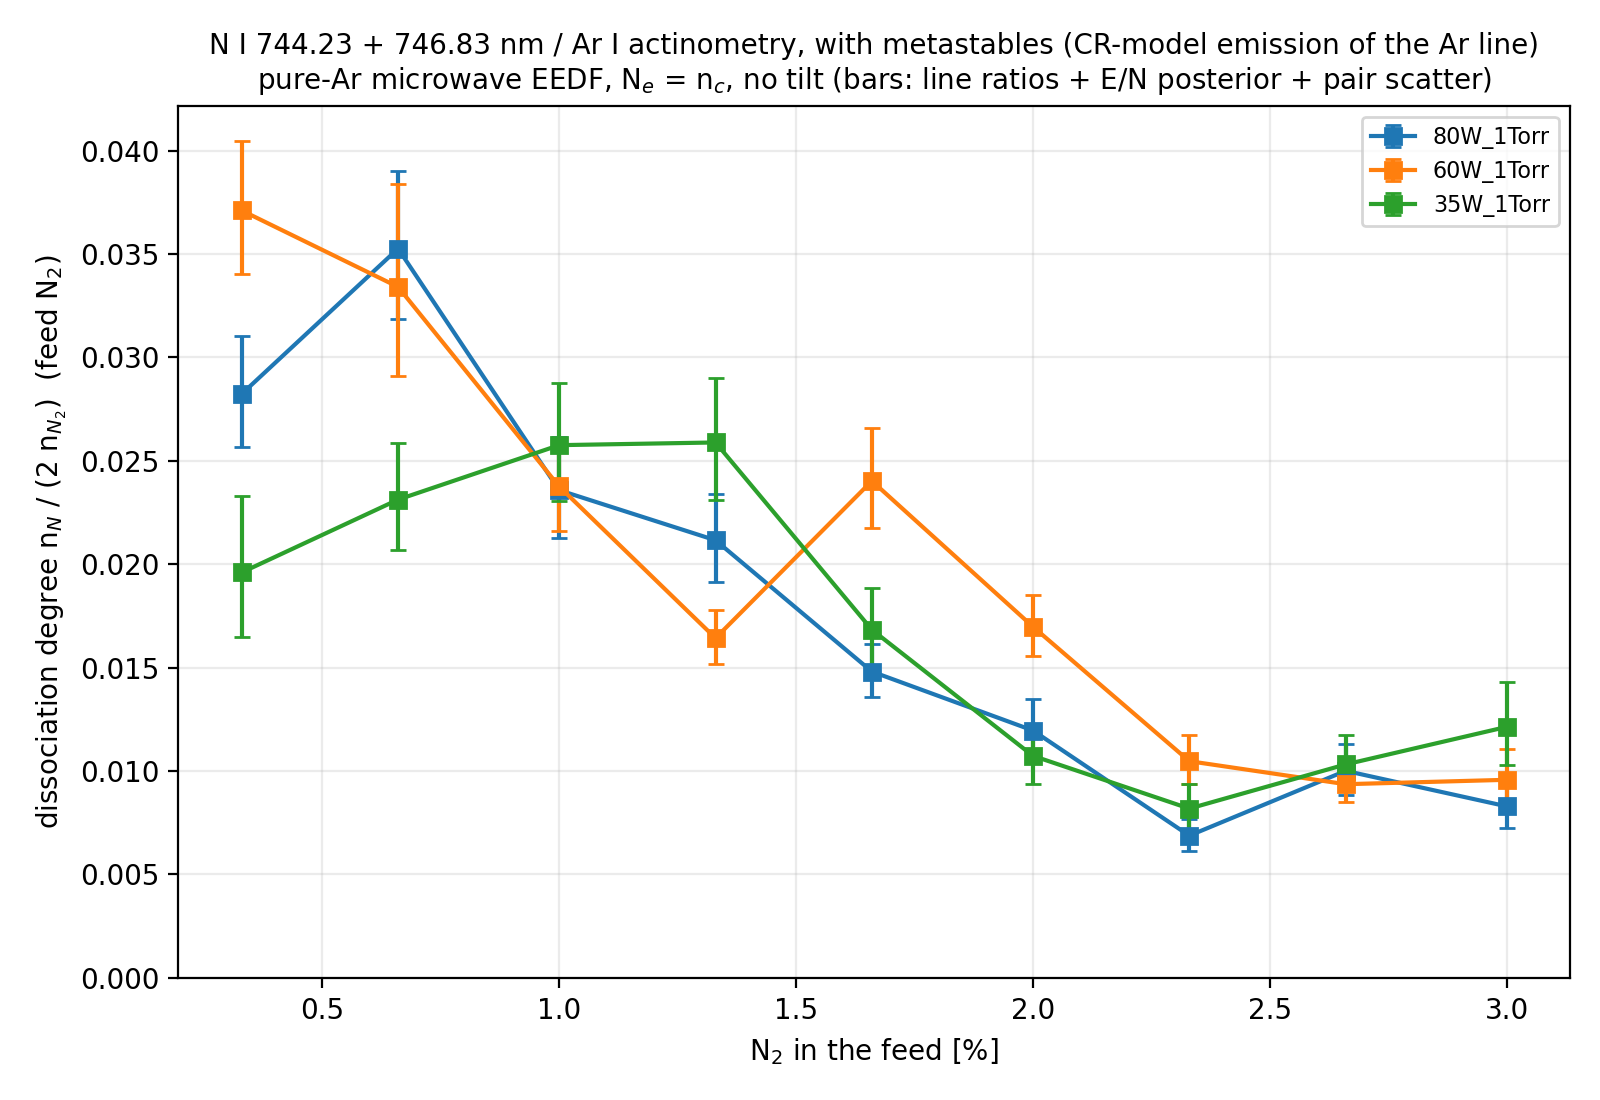
\includegraphics[width=0.49\linewidth]{ov_N2_dissociation}
\caption{$n_N/n_{Ar}$ (left) and dissociation degree (right) with metastables, all pairs combined, for the three
N$_2$ sweeps.}
\label{fig:actN2}
\end{figure}

\begin{figure}[H]
\centering
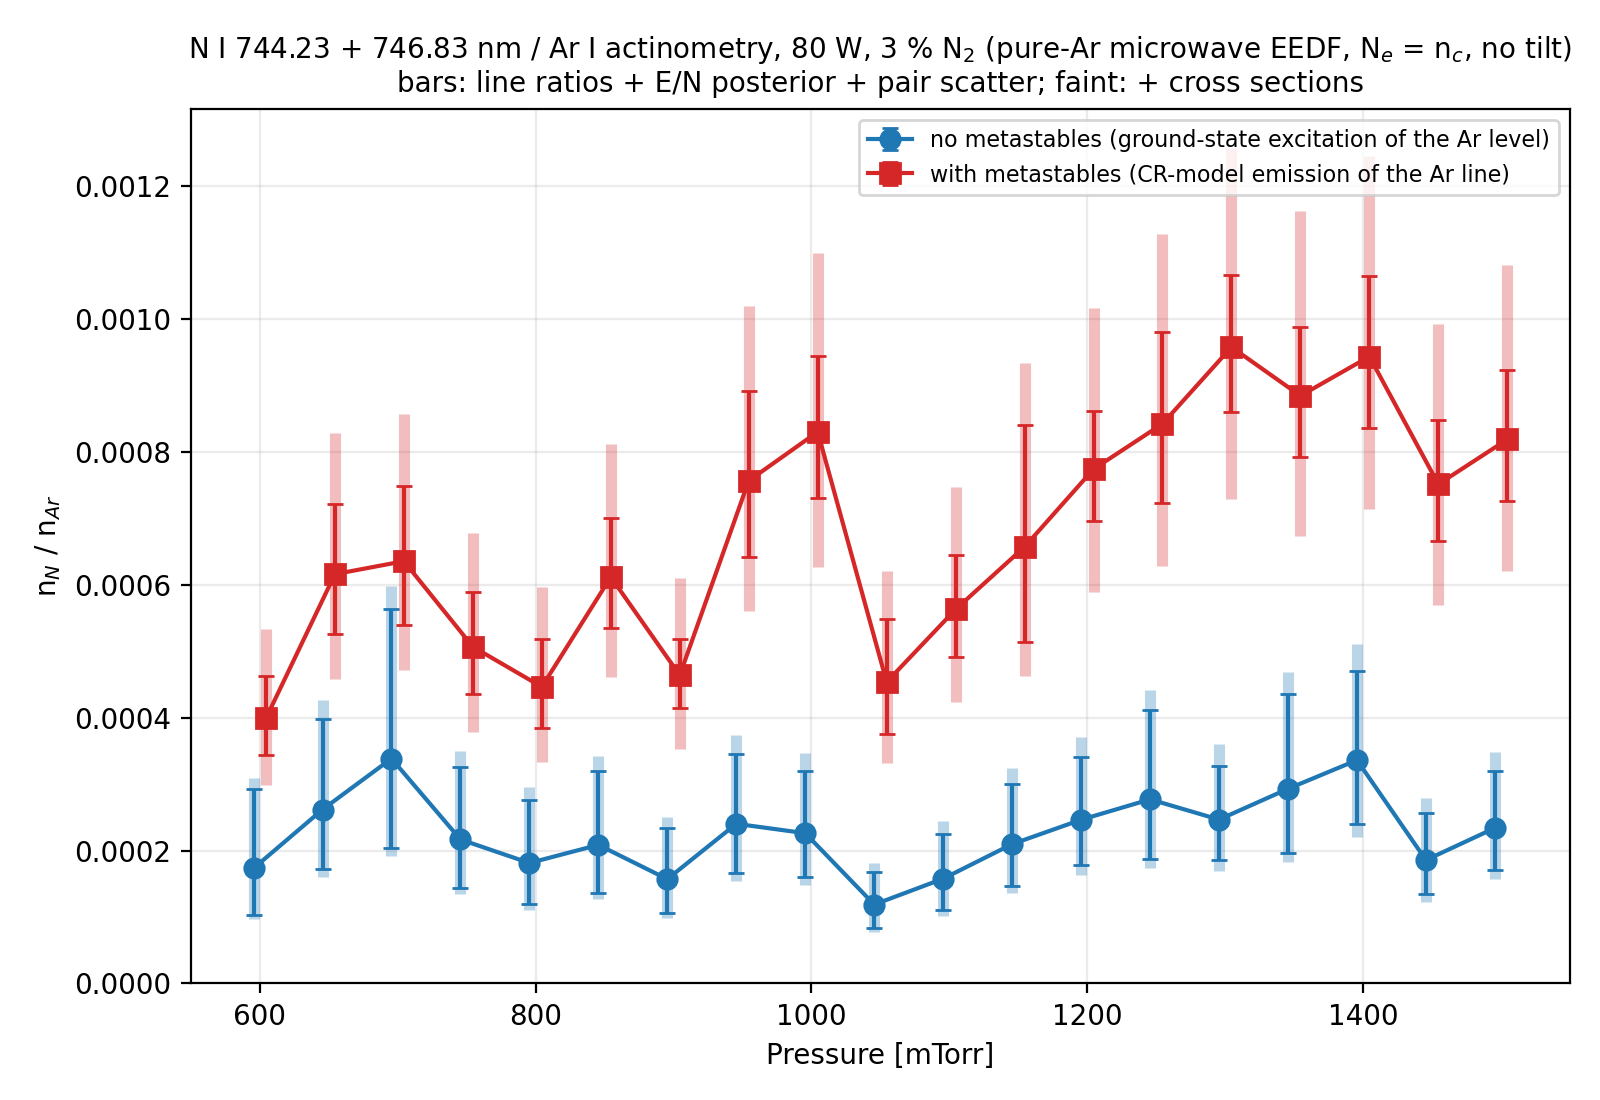
\includegraphics[width=0.49\linewidth]{p_actinometry}\hfill
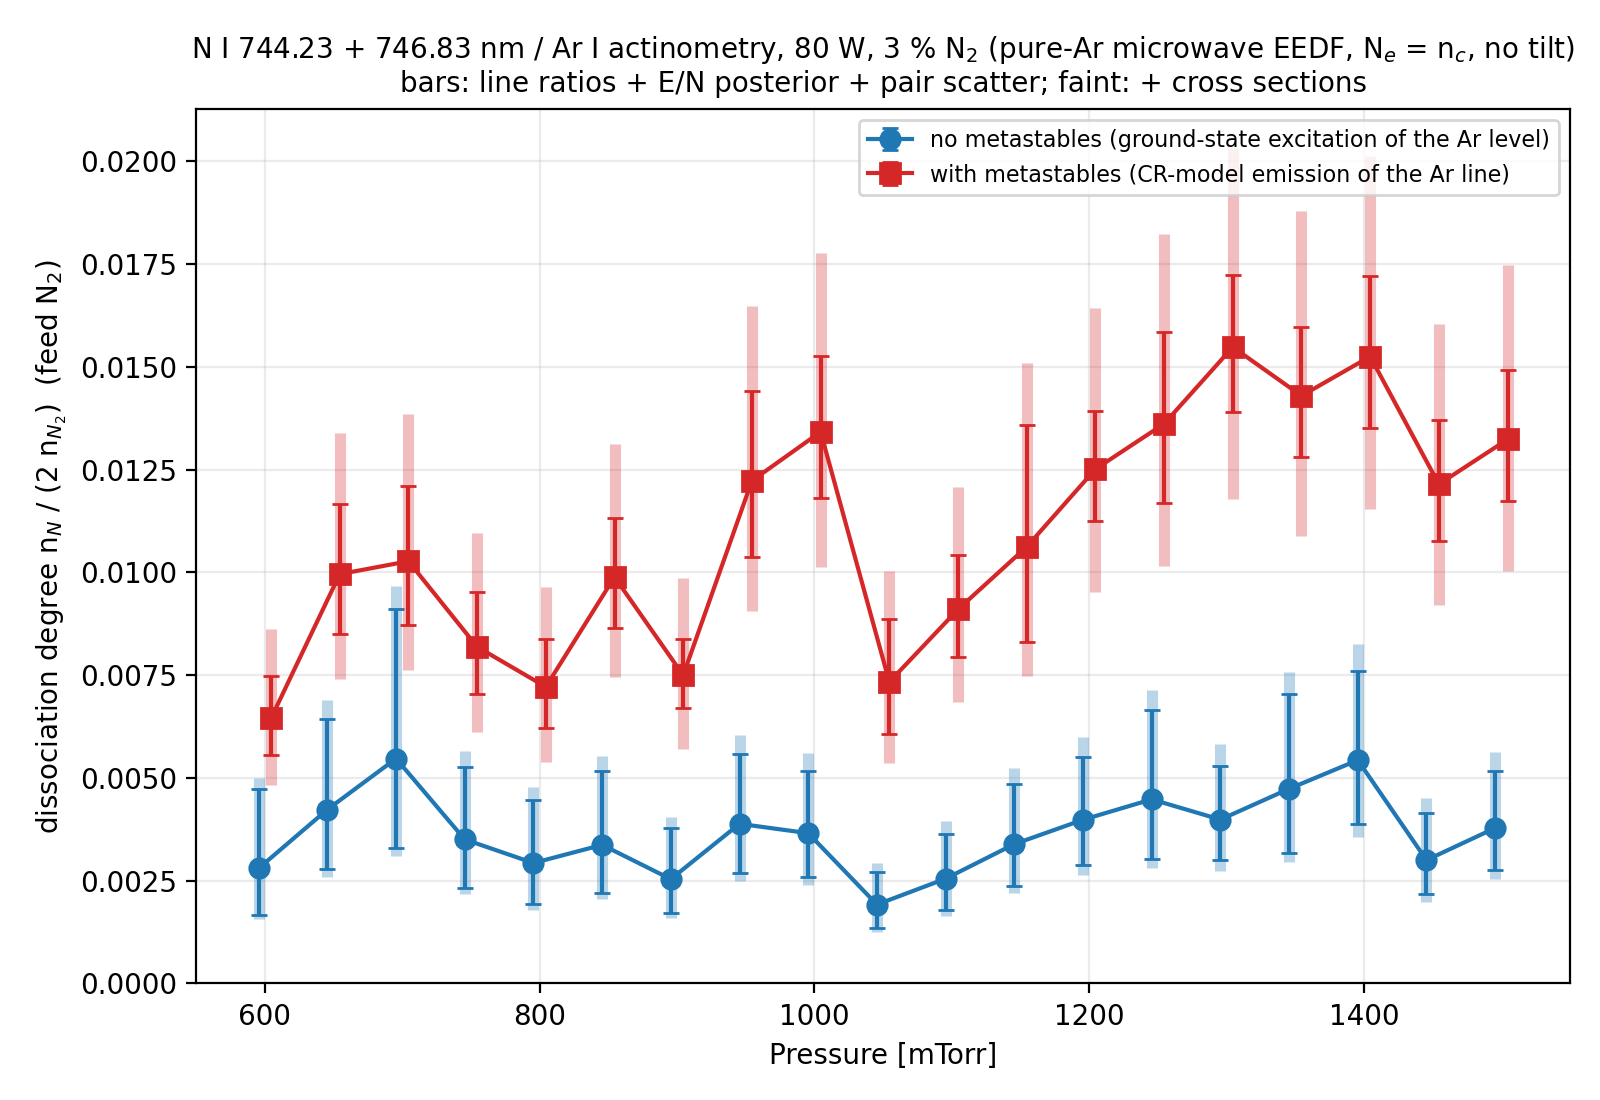
\includegraphics[width=0.49\linewidth]{p_dissociation}
\caption{As Fig.~\ref{fig:actN2} for the pressure sweep (80\,W, 3\,\% N$_2$); both variants.}
\label{fig:actp}
\end{figure}

\begin{figure}[H]
\centering
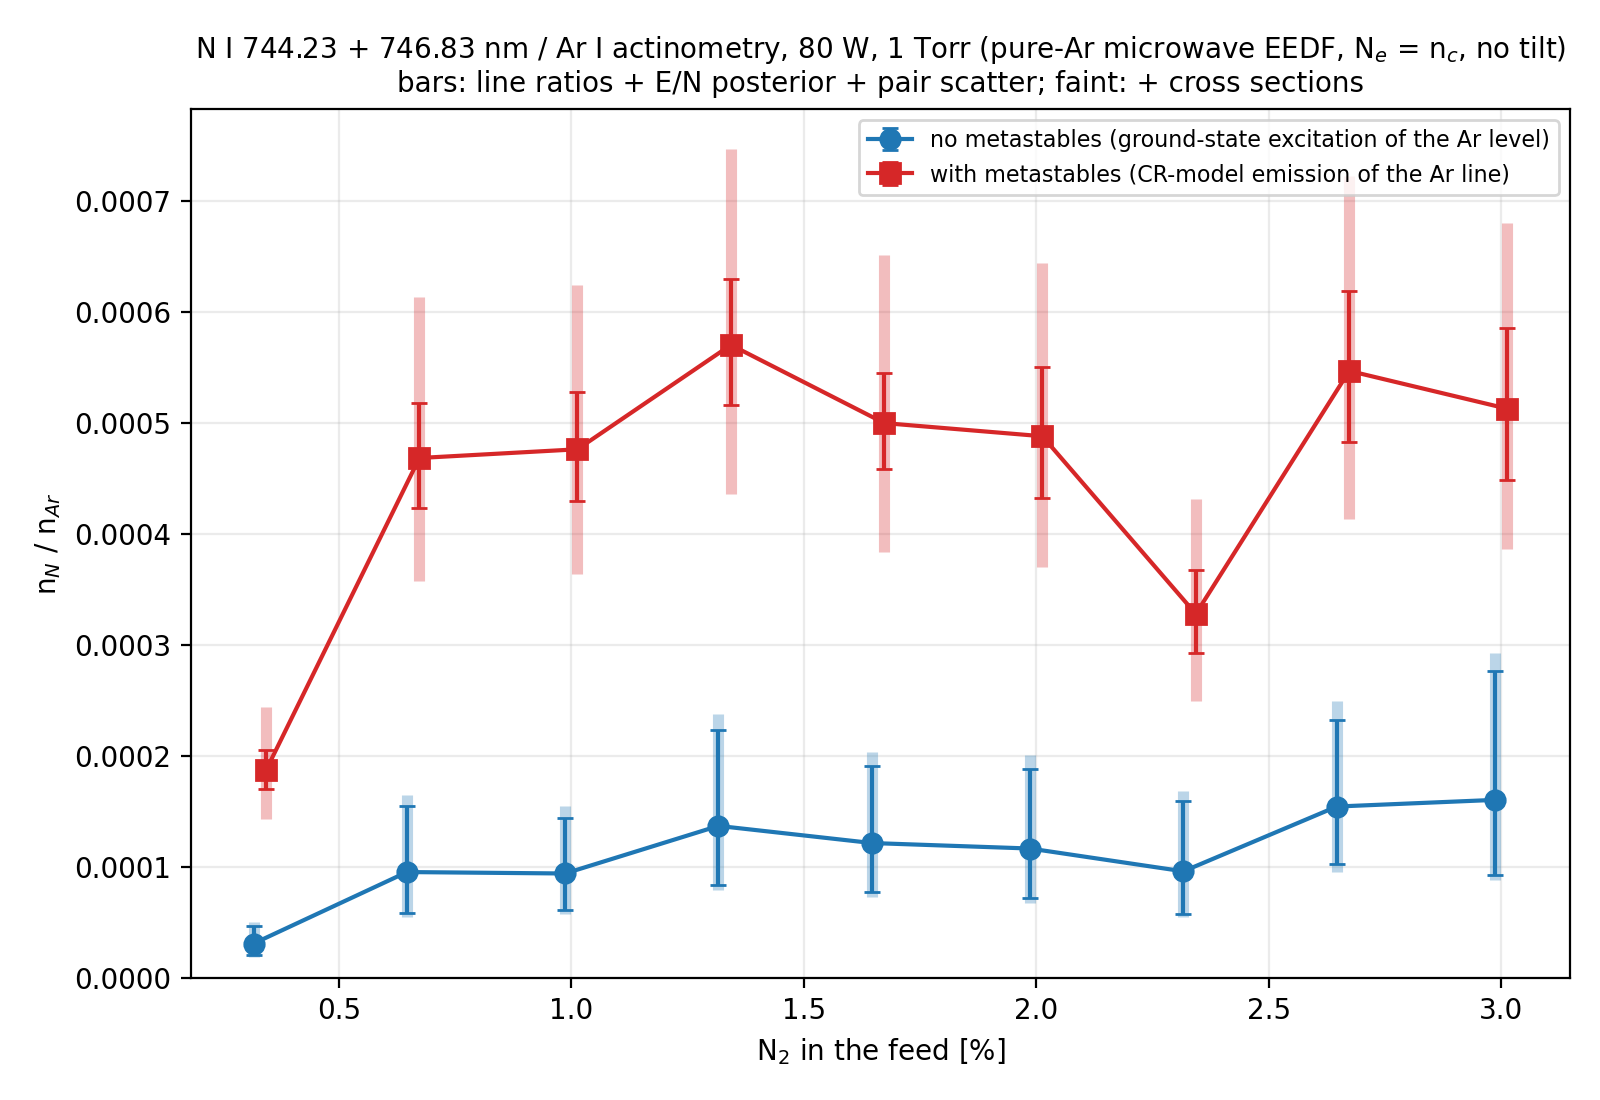
\includegraphics[width=0.49\linewidth]{80W_actinometry_variants}\hfill
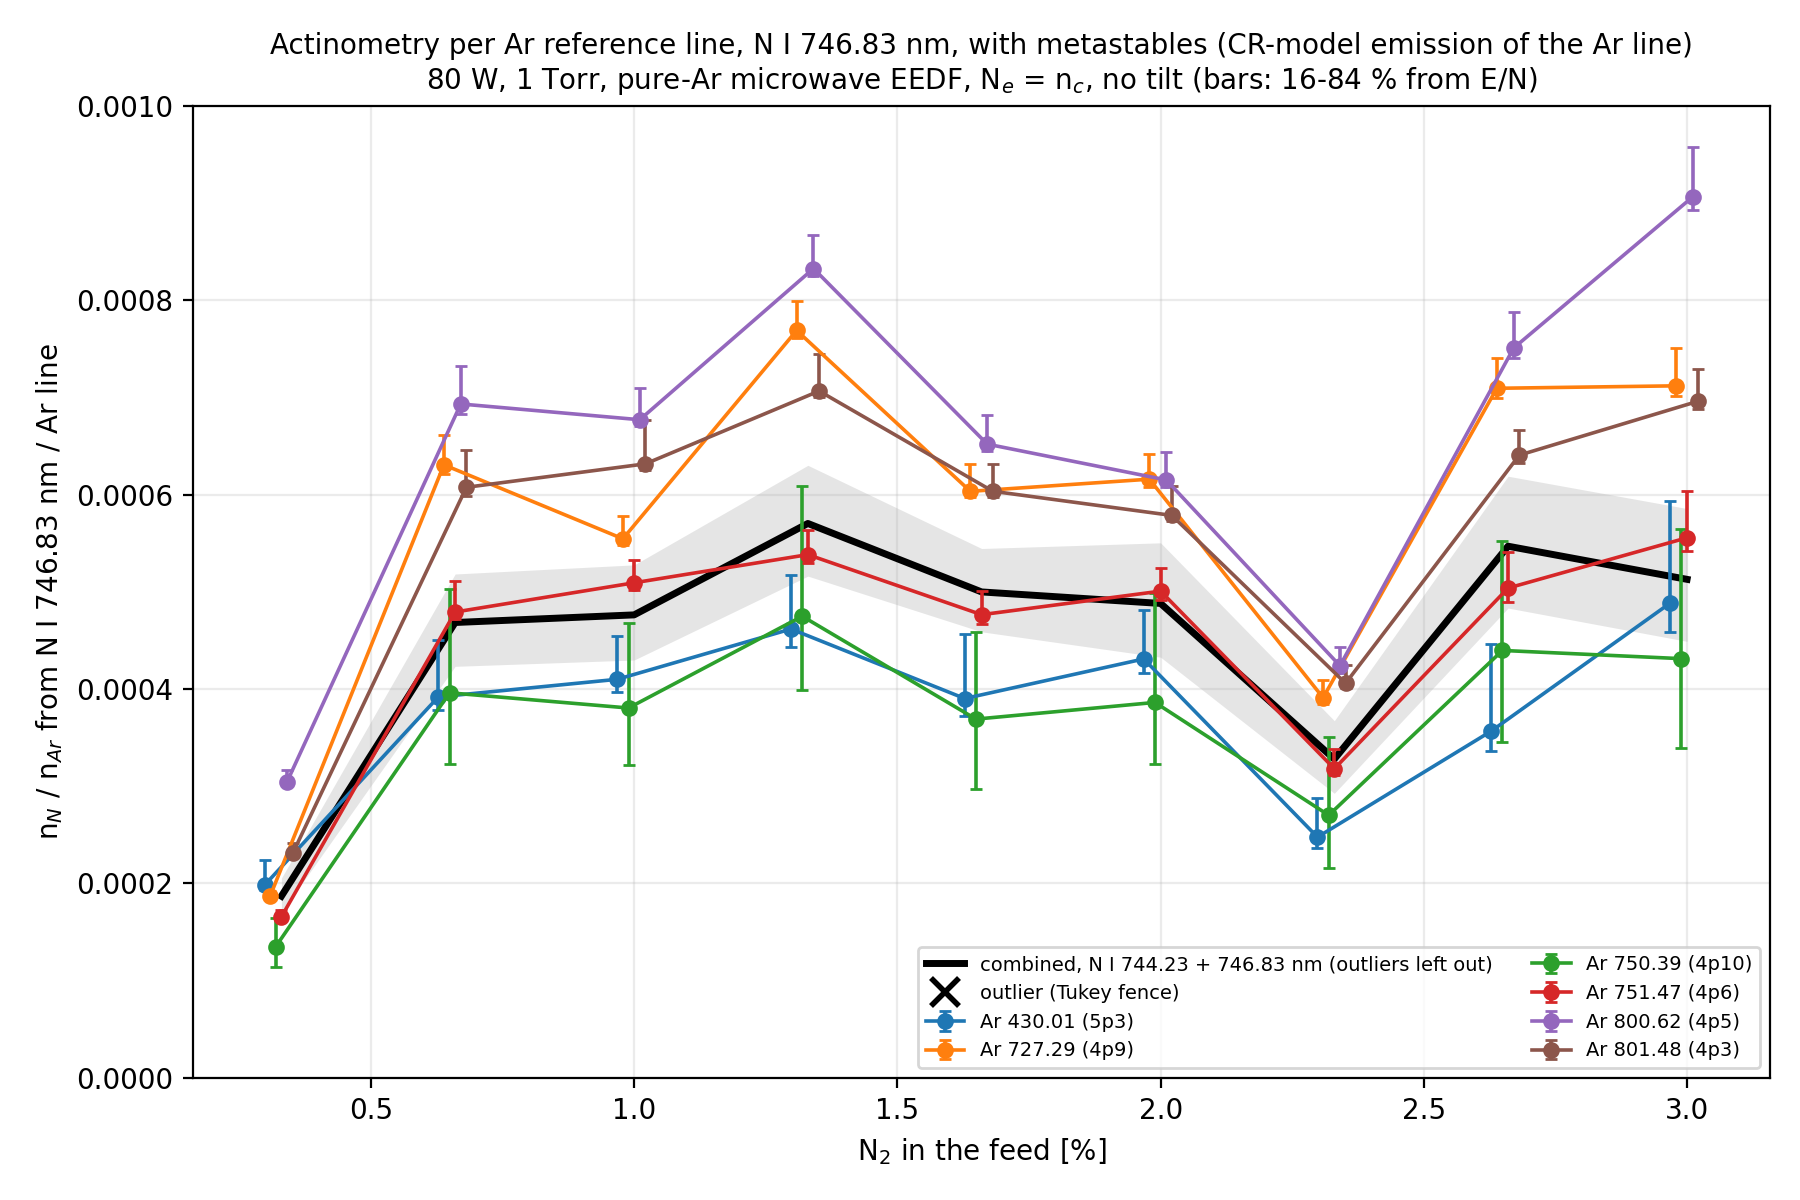
\includegraphics[width=0.49\linewidth]{80W_per_line_NI746p83}
\caption{80\,W, 1\,Torr. Left: both variants. Right: every N\,I\,746.83\,/\,Ar pair with metastables; black:
combined estimate, crosses: Tukey outliers.}
\label{fig:variants}
\end{figure}

\begin{figure}[H]
\centering
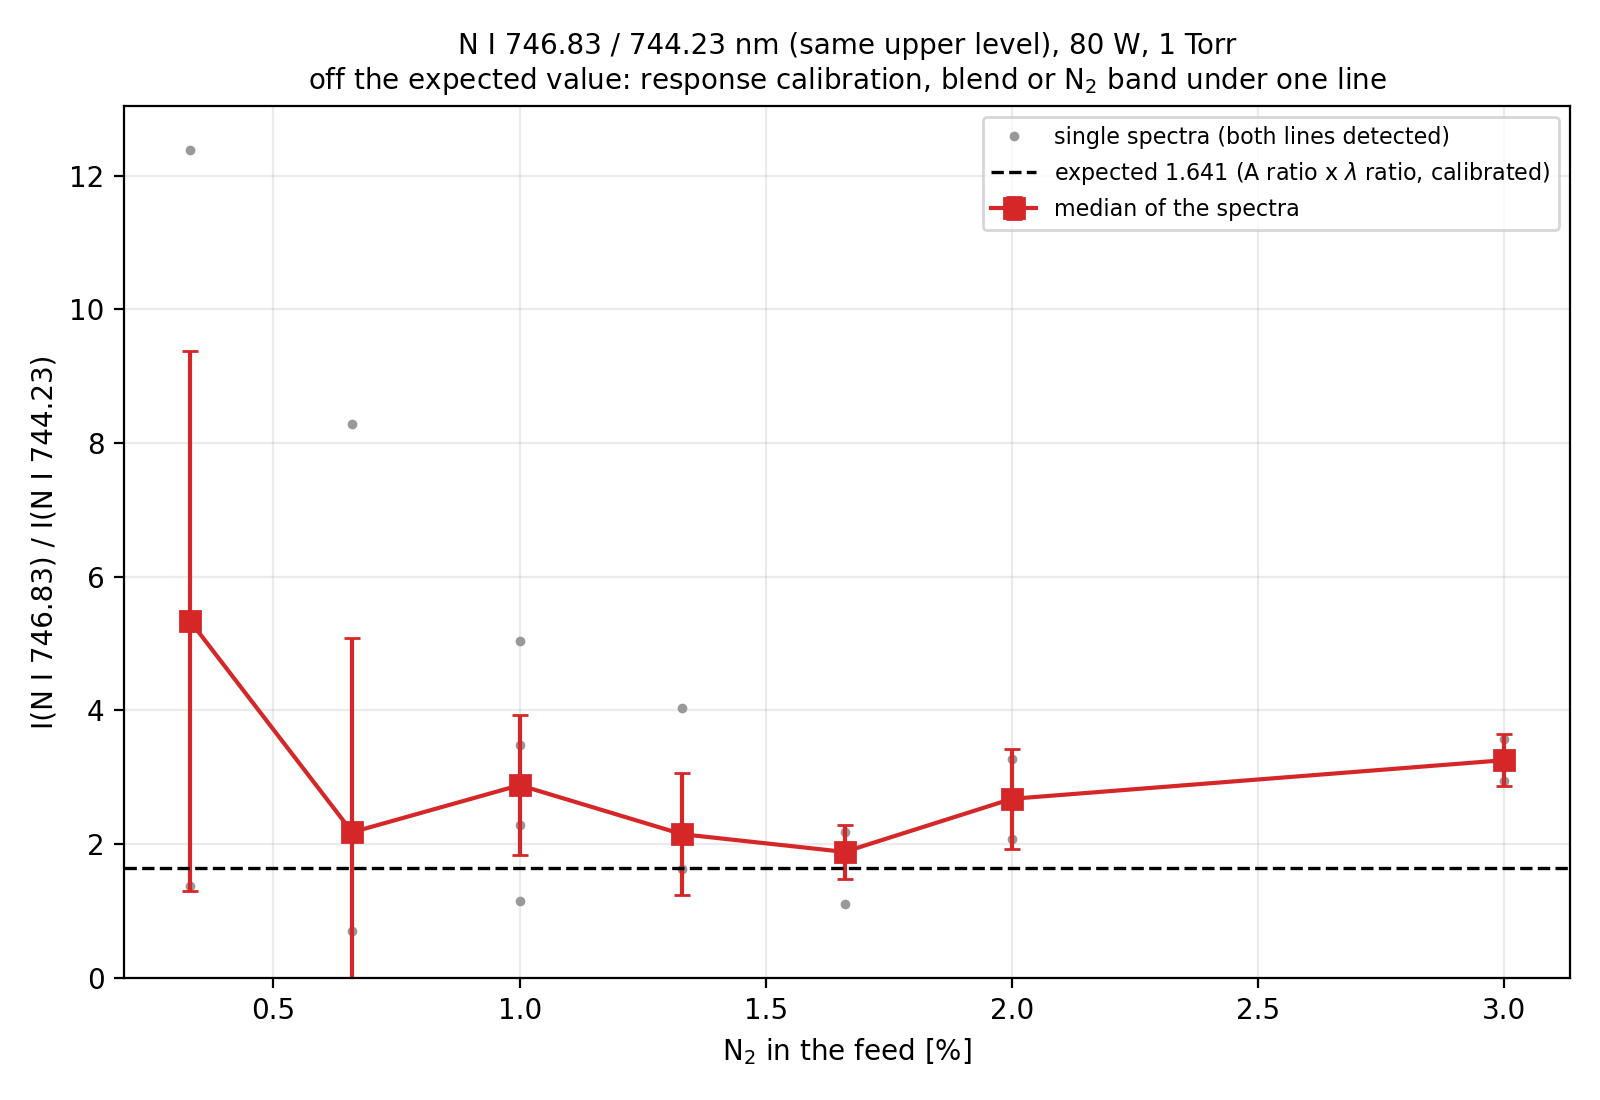
\includegraphics[width=0.49\linewidth]{80W_NI_same_upper}\hfill
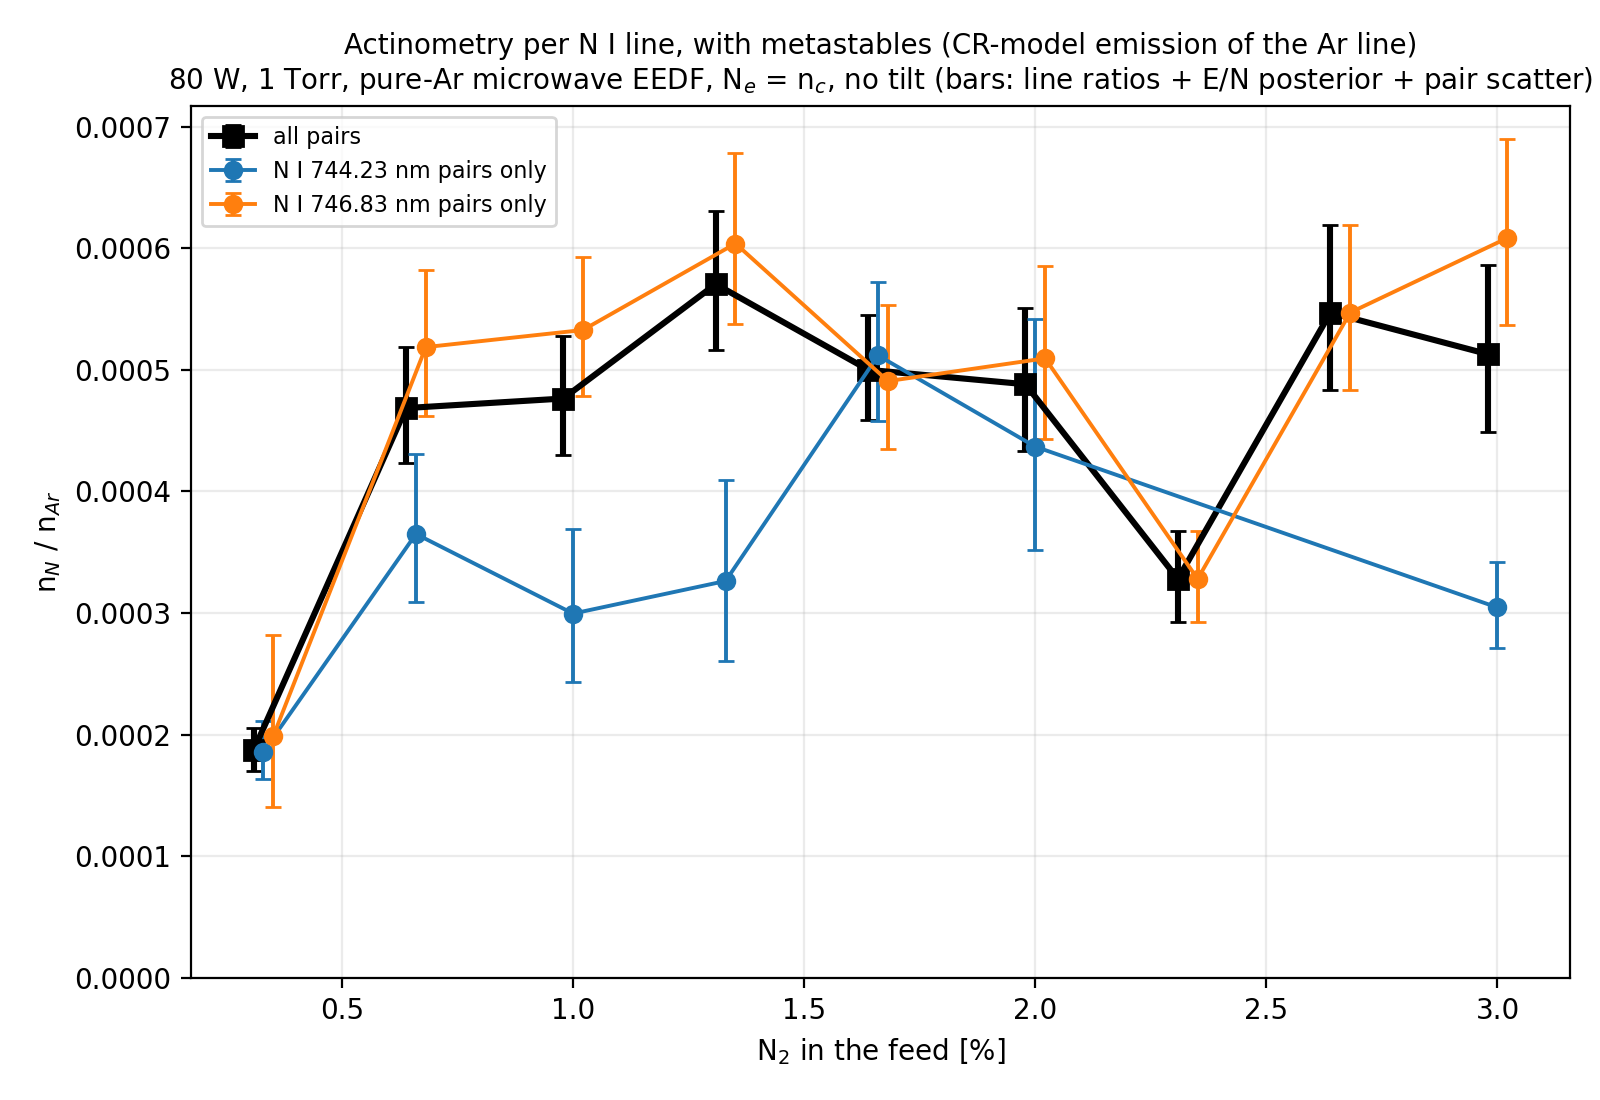
\includegraphics[width=0.49\linewidth]{80W_by_N_line}
\caption{80\,W, 1\,Torr. Left: measured I(746.83)/I(744.23) against the $A/\lambda$ ratio of the common upper level.
Right: $n_N/n_{Ar}$ from each N\,I line alone and from all pairs.}
\label{fig:sameupper}
\end{figure}

\begin{figure}[H]
\centering
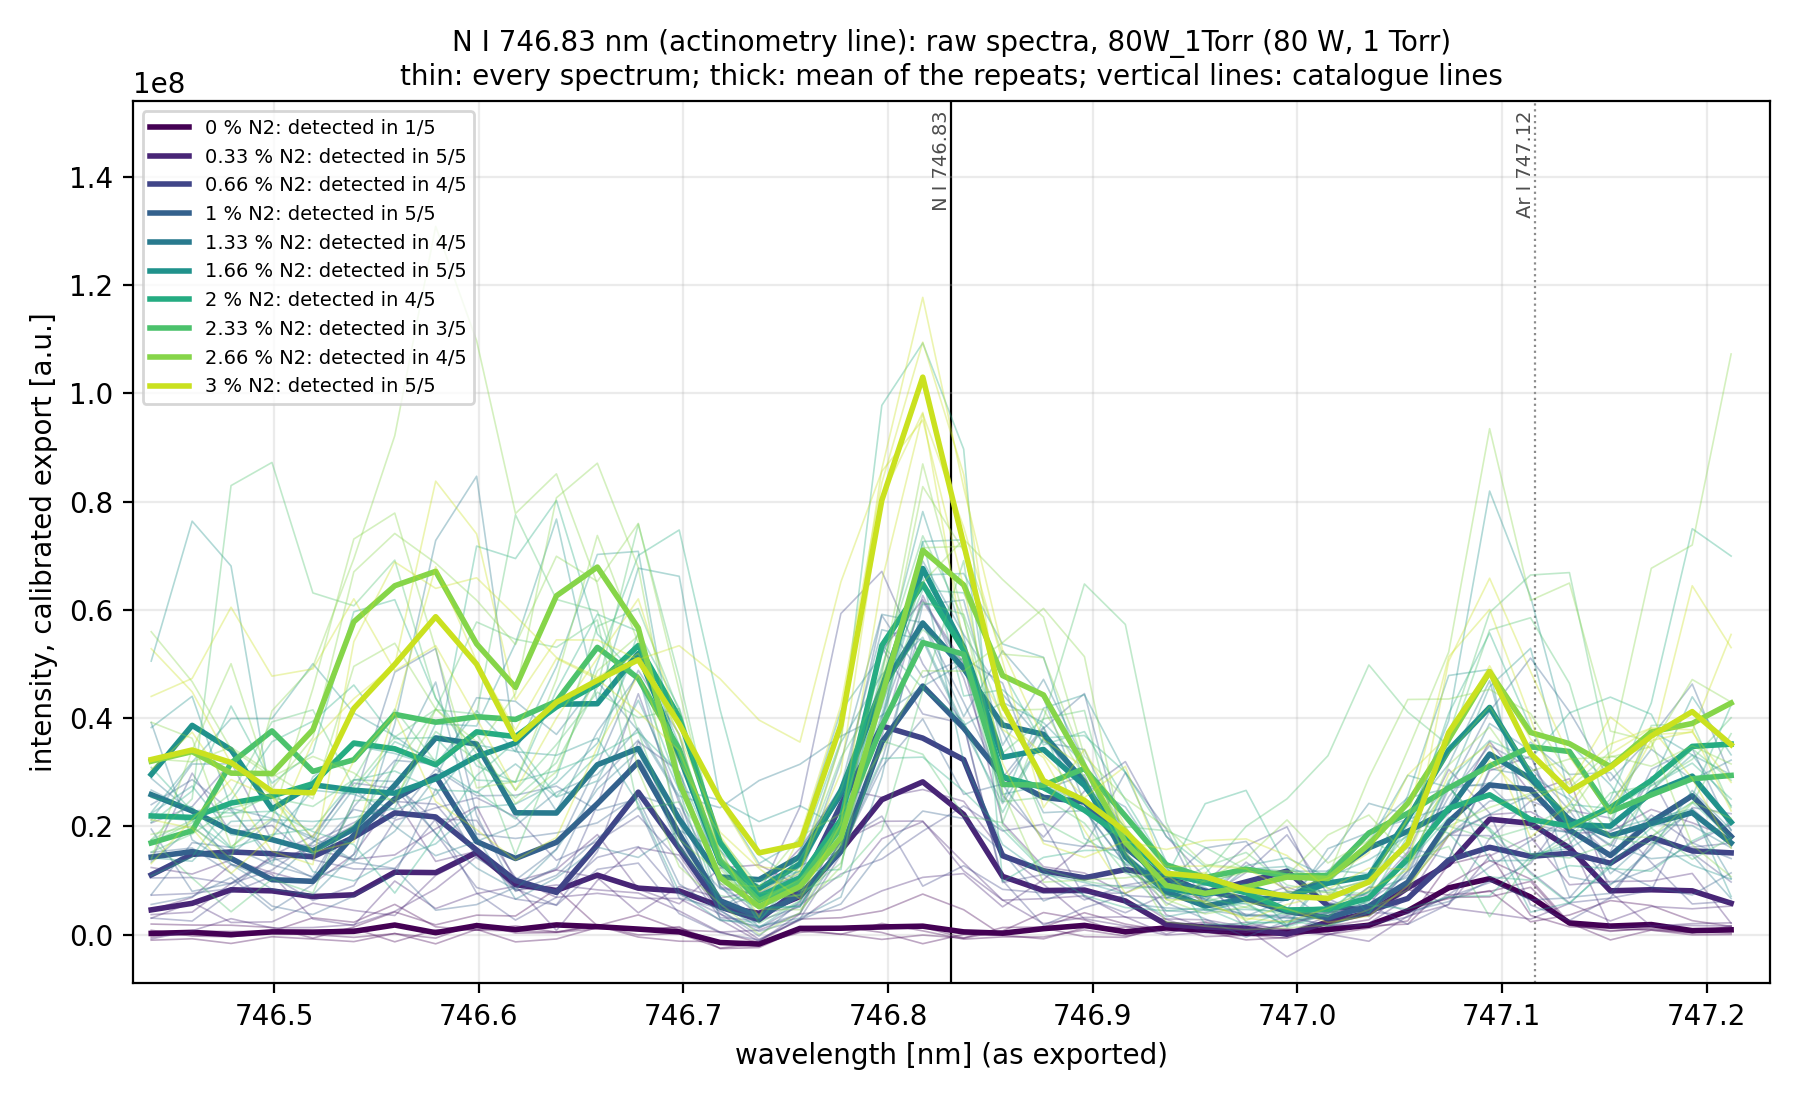
\includegraphics[width=0.49\linewidth]{80W_raw_NI746p83}\hfill
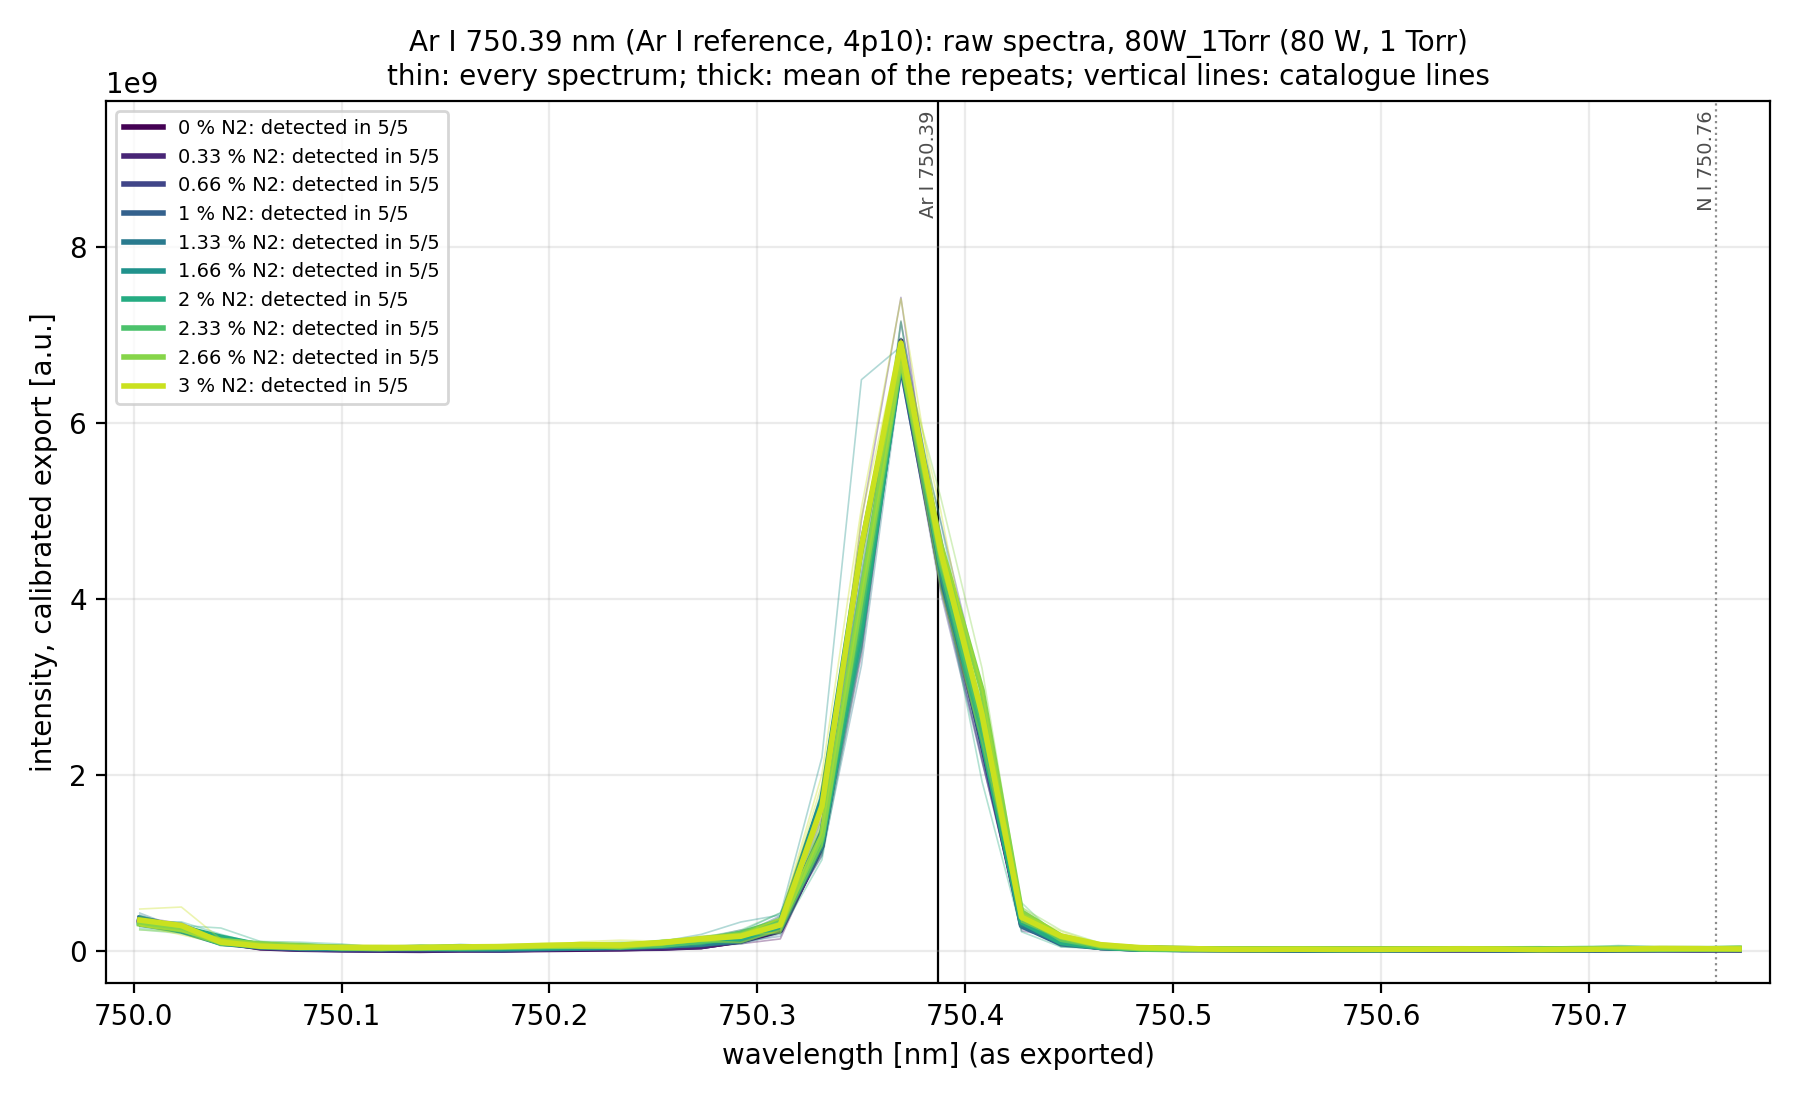
\includegraphics[width=0.49\linewidth]{80W_raw_ArI750p39}
\caption{Raw calibrated spectra of the 80\,W sweep around N\,I\,746.83\,nm (left) and the Ar\,I\,750.39\,nm reference
(right); thin: single spectra, thick: mean of the repeats; legend: number of spectra with the line detected.}
\label{fig:raw}
\end{figure}

%======================================================================================================
\section{Caveats and open points}
%======================================================================================================
\begin{itemize}
\item The pin at $\nc$ is an assumption (overdense discharge). At low N$_2$ fractions the lines alone prefer the dense branch, and at the lowest
  pressures of the 3\,\% sweep a density 3--4 times $\nc$, both by only a few $B^2$; elsewhere the free fit
  lands within a factor of 2--3 of $\nc$.
\item The EEDF ignores the N$_2$ (pure-Ar Boltzmann equation), chosen because the Ar/N$_2$ EEDF fails; why the real
  EEDF behaves like the pure-Ar one is open.
\item The CR 1s$_5$ falls faster with N$_2$ than LAS (CR/LAS down to 0.36 at 3\,\%): the N$_2$ quenching rates of
  the 4s levels (median of the literature values) need checking.
\item N\,I is excited from ground-state N only; any dissociative excitation would make $n_N$ an overestimate.
\item The per-spectrum scales of the repeats agree within about 5\,\%. A scale shared by all spectra of a sweep would
  add the change of the absolute intensities as information, which the present fit discards.
\item CR tables from the 2026-10-07 model (pooling on every level, two-body Ar quenching); effect $<2\,\%$.
\end{itemize}

\appendix
\section{Tables}
\small
egingroupootnotesize
\begin{longtable}{p{0.42\linewidth}rrrp{0.30\linewidth}}
\caption{BOLSIG+ libraries (pure Ar, 2.42\,GHz, Biagi cross sections, 42 E/N rows from 3 to 1000\,Td) and the conditions that use them. One CR table per library and N$_2$ fraction (column N$_2$: number of tables).}\label{tab:libraries}\\
\toprule library & $p$ [mTorr] & $T_g$ [K] & N$_2$ & conditions (sweep values) \\ \midrule\endfirsthead
\toprule library & $p$ [mTorr] & $T_g$ [K] & N$_2$ & conditions (sweep values) \\ \midrule\endhead
\texttt{Ar\_Biagi\_bolsig\_mw2.42GHz\_650K\_600mTorr} & 600 & 650 & 1 & 80W\_3pctN2\_pressure: 600 \\
\texttt{Ar\_Biagi\_bolsig\_mw2.42GHz\_650K\_650mTorr} & 650 & 650 & 1 & 80W\_3pctN2\_pressure: 650 \\
\texttt{Ar\_Biagi\_bolsig\_mw2.42GHz\_650K\_700mTorr} & 700 & 650 & 1 & 80W\_3pctN2\_pressure: 700 \\
\texttt{Ar\_Biagi\_bolsig\_mw2.42GHz\_650K\_750mTorr} & 750 & 650 & 1 & 80W\_3pctN2\_pressure: 750 \\
\texttt{Ar\_Biagi\_bolsig\_mw2.42GHz\_700K\_800mTorr} & 800 & 700 & 1 & 80W\_3pctN2\_pressure: 800 \\
\texttt{Ar\_Biagi\_bolsig\_mw2.42GHz\_700K\_850mTorr} & 850 & 700 & 1 & 80W\_3pctN2\_pressure: 850 \\
\texttt{Ar\_Biagi\_bolsig\_mw2.42GHz\_700K\_900mTorr} & 900 & 700 & 1 & 80W\_3pctN2\_pressure: 900 \\
\texttt{Ar\_Biagi\_bolsig\_mw2.42GHz\_700K\_950mTorr} & 950 & 700 & 1 & 80W\_3pctN2\_pressure: 950 \\
\texttt{Ar\_Biagi\_bolsig\_mw2.42GHz\_600K\_1000mTorr} & 1000 & 600 & 2 & 35W\_1Torr: 0, 0.33 \\
\texttt{Ar\_Biagi\_bolsig\_mw2.42GHz\_650K\_1000mTorr} & 1000 & 650 & 9 & 80W\_1Torr: 0, 0.33, 0.66; 60W\_1Torr: 0, 0.33, 0.66, 1, 1.33, 1.66; 35W\_1Torr: 0.66, 1, 1.33, 1.66, 2, 2.33, 2.66 \\
\texttt{Ar\_Biagi\_bolsig\_mw2.42GHz\_700K\_1000mTorr} & 1000 & 700 & 7 & 80W\_1Torr: 1, 1.33, 1.66, 2, 2.33, 2.66, 3; 60W\_1Torr: 2, 2.33, 2.66, 3; 35W\_1Torr: 3; 80W\_3pctN2\_pressure: 1000 \\
\texttt{Ar\_Biagi\_bolsig\_mw2.42GHz\_750K\_1050mTorr} & 1050 & 750 & 1 & 80W\_3pctN2\_pressure: 1050 \\
\texttt{Ar\_Biagi\_bolsig\_mw2.42GHz\_750K\_1100mTorr} & 1100 & 750 & 1 & 80W\_3pctN2\_pressure: 1100 \\
\texttt{Ar\_Biagi\_bolsig\_mw2.42GHz\_750K\_1150mTorr} & 1150 & 750 & 1 & 80W\_3pctN2\_pressure: 1150 \\
\texttt{Ar\_Biagi\_bolsig\_mw2.42GHz\_750K\_1200mTorr} & 1200 & 750 & 1 & 80W\_3pctN2\_pressure: 1200 \\
\texttt{Ar\_Biagi\_bolsig\_mw2.42GHz\_750K\_1250mTorr} & 1250 & 750 & 1 & 80W\_3pctN2\_pressure: 1250 \\
\texttt{Ar\_Biagi\_bolsig\_mw2.42GHz\_750K\_1300mTorr} & 1300 & 750 & 1 & 80W\_3pctN2\_pressure: 1300 \\
\texttt{Ar\_Biagi\_bolsig\_mw2.42GHz\_800K\_1350mTorr} & 1350 & 800 & 1 & 80W\_3pctN2\_pressure: 1350 \\
\texttt{Ar\_Biagi\_bolsig\_mw2.42GHz\_800K\_1400mTorr} & 1400 & 800 & 1 & 80W\_3pctN2\_pressure: 1400 \\
\texttt{Ar\_Biagi\_bolsig\_mw2.42GHz\_800K\_1450mTorr} & 1450 & 800 & 1 & 80W\_3pctN2\_pressure: 1450 \\
\texttt{Ar\_Biagi\_bolsig\_mw2.42GHz\_800K\_1500mTorr} & 1500 & 800 & 1 & 80W\_3pctN2\_pressure: 1500 \\
\bottomrule
\end{longtable}
\endgroup

\begin{longtable}{rrlrrrrrr}
\caption{CR fit of every condition: pinned at $n_c$ (E/N with its $\Delta\chi^2\le B^2$ band, $T_{e,\mathrm{eff}}$, $\chi^2$ per degree of freedom), the cost of the pin and the free fit. $x$: \% N$_2$ or pressure in mTorr.}\label{tab:fits}\\
\toprule $x$ & $T_g$ [K] & E/N at $n_c$ [Td] & $T_{e,\mathrm{eff}}$ [eV] & $\chi^2_\nu(n_c)$ & $\Delta\chi^2/B^2$ & $N_e$ free [m$^{-3}$] & $\chi^2_\nu$ free & 1s$_5$ CR/LAS \\ \endfirsthead
\toprule $x$ & $T_g$ [K] & E/N at $n_c$ [Td] & $T_{e,\mathrm{eff}}$ [eV] & $\chi^2_\nu(n_c)$ & $\Delta\chi^2/B^2$ & $N_e$ free [m$^{-3}$] & $\chi^2_\nu$ free & 1s$_5$ CR/LAS \\ \endhead
\midrule\multicolumn{9}{l}{\textbf{80W\_1Torr}}\\
0 & 650 & 36.2 [31.9, 41.2] & 0.809 & 1.82 & 8.4 & $3.0\times10^{19}$ & 1.53 & 0.86 \\
0.33 & 650 & 35.5 [31.9, 40.3] & 0.808 & 1.63 & 6.8 & $3.0\times10^{19}$ & 1.42 & 0.69 \\
0.66 & 650 & 35.5 [30.5, 40.3] & 0.808 & 1.87 & 5.2 & $3.0\times10^{19}$ & 1.69 & 0.60 \\
1 & 700 & 36.2 [32.6, 41.2] & 0.807 & 1.66 & 3.2 & $3.0\times10^{19}$ & 1.57 & 0.43 \\
1.33 & 700 & 36.2 [32.6, 41.2] & 0.807 & 1.44 & 2.7 & $3.0\times10^{19}$ & 1.38 & 0.41 \\
1.66 & 700 & 37.0 [32.6, 42.1] & 0.807 & 1.83 & 0.6 & $1.4\times10^{17}$ & 1.84 & 0.41 \\
2 & 700 & 35.5 [31.9, 41.2] & 0.807 & 1.53 & 1.0 & $1.5\times10^{17}$ & 1.53 & 0.35 \\
2.33 & 700 & 36.2 [31.9, 42.1] & 0.807 & 1.76 & 1.5 & $1.8\times10^{17}$ & 1.74 & 0.36 \\
2.66 & 700 & 37.8 [32.6, 43.9] & 0.808 & 1.80 & 1.6 & $1.7\times10^{17}$ & 1.77 & 0.39 \\
3 & 700 & 37.0 [31.9, 43.0] & 0.807 & 1.85 & 0.9 & $1.5\times10^{17}$ & 1.86 & 0.36 \\
\midrule\multicolumn{9}{l}{\textbf{60W\_1Torr}}\\
0 & 650 & 37.0 [31.2, 43.9] & 0.811 & 3.04 & 5.7 & $3.0\times10^{19}$ & 2.71 & 0.90 \\
0.33 & 650 & 34.7 [30.5, 39.5] & 0.807 & 1.77 & 6.8 & $3.0\times10^{19}$ & 1.54 & 0.64 \\
0.66 & 650 & 35.5 [31.2, 39.5] & 0.808 & 1.52 & 4.9 & $3.0\times10^{19}$ & 1.38 & 0.59 \\
1 & 650 & 34.7 [29.9, 39.5] & 0.807 & 1.67 & 2.9 & $3.0\times10^{19}$ & 1.59 & 0.49 \\
1.33 & 650 & 34.7 [29.9, 39.5] & 0.807 & 1.61 & 1.6 & $2.0\times10^{17}$ & 1.59 & 0.49 \\
1.66 & 650 & 34.7 [30.5, 39.5] & 0.807 & 1.64 & 0.7 & $3.0\times10^{19}$ & 1.65 & 0.48 \\
2 & 700 & 37.8 [33.3, 43.0] & 0.808 & 1.52 & 1.6 & $1.7\times10^{17}$ & 1.50 & 0.48 \\
2.33 & 700 & 38.6 [33.3, 43.9] & 0.808 & 1.55 & 2.3 & $2.2\times10^{17}$ & 1.50 & 0.50 \\
2.66 & 700 & 37.0 [33.3, 41.2] & 0.807 & 1.16 & 2.0 & $1.6\times10^{17}$ & 1.13 & 0.44 \\
3 & 700 & 38.6 [34.0, 43.9] & 0.808 & 1.56 & 1.2 & $1.5\times10^{17}$ & 1.55 & 0.50 \\
\midrule\multicolumn{9}{l}{\textbf{35W\_1Torr}}\\
0 & 600 & 32.6 [28.6, 37.8] & 0.812 & 1.79 & 10.8 & $3.0\times10^{19}$ & 1.43 & 0.84 \\
0.33 & 600 & 31.9 [28.0, 37.0] & 0.811 & 2.06 & 3.8 & $3.0\times10^{19}$ & 1.93 & 0.66 \\
0.66 & 650 & 36.2 [31.9, 40.3] & 0.809 & 1.68 & 3.4 & $3.0\times10^{19}$ & 1.59 & 0.62 \\
1 & 650 & 36.2 [31.2, 41.2] & 0.809 & 1.86 & 1.0 & $1.9\times10^{17}$ & 1.86 & 0.54 \\
1.33 & 650 & 38.6 [34.7, 43.0] & 0.814 & 1.37 & 1.1 & $1.7\times10^{17}$ & 1.36 & 0.65 \\
1.66 & 650 & 37.0 [32.6, 43.0] & 0.811 & 1.79 & 1.5 & $2.0\times10^{17}$ & 1.77 & 0.58 \\
2 & 650 & 37.0 [32.6, 42.1] & 0.811 & 1.69 & 0.4 & $1.2\times10^{17}$ & 1.72 & 0.58 \\
2.33 & 650 & 41.2 [36.2, 46.8] & 0.822 & 1.58 & 1.0 & $1.5\times10^{17}$ & 1.59 & 0.78 \\
2.66 & 650 & 39.5 [34.7, 43.9] & 0.816 & 1.60 & 0.3 & $1.1\times10^{17}$ & 1.63 & 0.69 \\
3 & 700 & 43.9 [38.6, 48.9] & 0.820 & 1.63 & 0.5 & $1.2\times10^{17}$ & 1.65 & 0.74 \\
\midrule\multicolumn{9}{l}{\textbf{80W\_3pctN2\_pressure}}\\
600 & 650 & 62.1 [54.1, 69.9] & 0.806 & 1.34 & 5.7 & $2.8\times10^{17}$ & 1.19 & 0.23 \\
650 & 650 & 62.1 [55.2, 69.9] & 0.816 & 1.28 & 5.7 & $2.8\times10^{17}$ & 1.14 & 0.31 \\
700 & 650 & 54.5 [47.3, 61.6] & 0.808 & 1.53 & 3.6 & $2.4\times10^{17}$ & 1.44 & 0.29 \\
750 & 650 & 54.5 [47.3, 60.3] & 0.818 & 1.25 & 7.0 & $2.8\times10^{17}$ & 1.08 & 0.37 \\
800 & 700 & 49.3 [43.5, 54.7] & 0.805 & 1.23 & 3.5 & $2.0\times10^{17}$ & 1.15 & 0.28 \\
850 & 700 & 49.3 [42.6, 55.8] & 0.812 & 1.56 & 2.9 & $2.2\times10^{17}$ & 1.48 & 0.37 \\
900 & 700 & 43.5 [38.4, 49.3] & 0.807 & 1.41 & 1.6 & $1.5\times10^{17}$ & 1.39 & 0.34 \\
950 & 700 & 43.9 [37.8, 49.9] & 0.813 & 1.73 & 2.5 & $2.1\times10^{17}$ & 1.67 & 0.46 \\
1000 & 700 & 41.2 [35.5, 46.8] & 0.812 & 1.84 & 1.2 & $1.5\times10^{17}$ & 1.84 & 0.49 \\
1050 & 750 & 41.2 [35.5, 46.8] & 0.810 & 1.79 & 1.2 & $1.5\times10^{17}$ & 1.78 & 0.46 \\
1100 & 750 & 40.3 [34.7, 45.8] & 0.812 & 1.82 & 1.4 & $1.5\times10^{17}$ & 1.81 & 0.51 \\
1150 & 750 & 39.5 [35.5, 43.9] & 0.816 & 1.27 & 1.3 & $1.3\times10^{17}$ & 1.26 & 0.56 \\
1200 & 750 & 37.6 [33.6, 42.0] & 0.817 & 1.30 & 1.4 & $1.3\times10^{17}$ & 1.29 & 0.57 \\
1250 & 750 & 35.2 [30.8, 39.3] & 0.813 & 1.73 & 0.8 & $1.3\times10^{17}$ & 1.74 & 0.55 \\
1300 & 750 & 32.2 [28.8, 36.0] & 0.813 & 1.44 & 0.2 & $1.0\times10^{17}$ & 1.47 & 0.49 \\
1350 & 800 & 33.6 [29.5, 37.6] & 0.813 & 1.65 & 0.3 & $1.1\times10^{17}$ & 1.68 & 0.52 \\
1400 & 800 & 34.4 [30.8, 38.4] & 0.818 & 1.37 & 1.2 & $1.3\times10^{17}$ & 1.36 & 0.63 \\
1450 & 800 & 32.2 [28.2, 36.8] & 0.817 & 1.95 & 0.3 & $1.1\times10^{17}$ & 1.98 & 0.59 \\
1500 & 800 & 30.8 [27.6, 33.6] & 0.816 & 1.47 & 0.1 & $8.8\times10^{16}$ & 1.50 & 0.59 \\
\bottomrule
\end{longtable}

\begin{longtable}{rrrrrrr}
\caption{N I / Ar I actinometry at $n_c$, all pairs combined: with metastables (CR-model emission of the Ar line) and, last column, without (ground-state excitation only). $\sigma_{\ln}$: statistical error of $\ln(n_N/n_{Ar})$ (line ratios, E/N posterior, pair scatter); the cross sections add 0.25.}\label{tab:actinometry}\\
\toprule $x$ & pairs & $n_N/n_{Ar}$ (CR) & $\sigma_{\ln}$ stat & Birge & dissociation [\%] & $n_N/n_{Ar}$ (direct) \\ \endfirsthead
\toprule $x$ & pairs & $n_N/n_{Ar}$ (CR) & $\sigma_{\ln}$ stat & Birge & dissociation [\%] & $n_N/n_{Ar}$ (direct) \\ \endhead
\midrule\multicolumn{7}{l}{\textbf{80W\_1Torr}}\\
0.33 & 12 & $1.9\times10^{-4}$ & 0.09 & 0.94 & 2.82 & $3.1\times10^{-5}$ \\
0.66 & 12 & $4.7\times10^{-4}$ & 0.10 & 1.00 & 3.53 & $9.5\times10^{-5}$ \\
1 & 12 & $4.8\times10^{-4}$ & 0.10 & 1.06 & 2.36 & $9.4\times10^{-5}$ \\
1.33 & 12 & $5.7\times10^{-4}$ & 0.10 & 1.31 & 2.12 & $1.4\times10^{-4}$ \\
1.66 & 12 & $5.0\times10^{-4}$ & 0.09 & 1.13 & 1.48 & $1.2\times10^{-4}$ \\
2 & 12 & $4.9\times10^{-4}$ & 0.12 & 0.54 & 1.20 & $1.2\times10^{-4}$ \\
2.33 & 6 & $3.3\times10^{-4}$ & 0.11 & 1.54 & 0.69 & $9.6\times10^{-5}$ \\
2.66 & 6 & $5.5\times10^{-4}$ & 0.12 & 1.90 & 1.00 & $1.5\times10^{-4}$ \\
3 & 12 & $5.1\times10^{-4}$ & 0.13 & 2.44 & 0.83 & $1.6\times10^{-4}$ \\
\midrule\multicolumn{7}{l}{\textbf{60W\_1Torr}}\\
0.33 & 12 & $2.5\times10^{-4}$ & 0.09 & 1.68 & 3.71 & $4.2\times10^{-5}$ \\
0.66 & 12 & $4.4\times10^{-4}$ & 0.14 & 0.58 & 3.34 & $1.0\times10^{-4}$ \\
1 & 12 & $4.8\times10^{-4}$ & 0.09 & 0.73 & 2.38 & $1.0\times10^{-4}$ \\
1.33 & 12 & $4.4\times10^{-4}$ & 0.08 & 1.59 & 1.64 & $7.6\times10^{-5}$ \\
1.66 & 6 & $8.1\times10^{-4}$ & 0.10 & 1.00 & 2.40 & $2.7\times10^{-4}$ \\
2 & 10 & $6.9\times10^{-4}$ & 0.09 & 1.38 & 1.70 & $1.8\times10^{-4}$ \\
2.33 & 12 & $5.0\times10^{-4}$ & 0.11 & 0.83 & 1.05 & $1.3\times10^{-4}$ \\
2.66 & 12 & $5.1\times10^{-4}$ & 0.10 & 1.08 & 0.94 & $1.3\times10^{-4}$ \\
3 & 6 & $5.9\times10^{-4}$ & 0.15 & 2.15 & 0.96 & $2.0\times10^{-4}$ \\
\midrule\multicolumn{7}{l}{\textbf{35W\_1Torr}}\\
0.33 & 6 & $1.3\times10^{-4}$ & 0.17 & 0.51 & 1.96 & $2.1\times10^{-5}$ \\
0.66 & 12 & $3.1\times10^{-4}$ & 0.11 & 1.46 & 2.31 & $6.9\times10^{-5}$ \\
1 & 12 & $5.2\times10^{-4}$ & 0.11 & 1.04 & 2.58 & $1.1\times10^{-4}$ \\
1.33 & 12 & $7.0\times10^{-4}$ & 0.11 & 1.97 & 2.59 & $1.8\times10^{-4}$ \\
1.66 & 12 & $5.7\times10^{-4}$ & 0.11 & 0.89 & 1.68 & $1.4\times10^{-4}$ \\
2 & 6 & $4.4\times10^{-4}$ & 0.13 & 2.04 & 1.07 & $1.3\times10^{-4}$ \\
2.33 & 12 & $3.9\times10^{-4}$ & 0.14 & 1.03 & 0.82 & $1.2\times10^{-4}$ \\
2.66 & 12 & $5.6\times10^{-4}$ & 0.13 & 1.73 & 1.03 & $1.7\times10^{-4}$ \\
3 & 12 & $7.5\times10^{-4}$ & 0.16 & 1.09 & 1.21 & $2.2\times10^{-4}$ \\
\midrule\multicolumn{7}{l}{\textbf{80W\_3pctN2\_pressure}}\\
600 & 12 & $4.0\times10^{-4}$ & 0.15 & 0.69 & 0.64 & $1.7\times10^{-4}$ \\
650 & 12 & $6.2\times10^{-4}$ & 0.16 & 0.70 & 1.00 & $2.6\times10^{-4}$ \\
700 & 12 & $6.4\times10^{-4}$ & 0.16 & 3.17 & 1.03 & $3.4\times10^{-4}$ \\
750 & 12 & $5.1\times10^{-4}$ & 0.15 & 3.08 & 0.82 & $2.2\times10^{-4}$ \\
800 & 12 & $4.5\times10^{-4}$ & 0.15 & 0.42 & 0.72 & $1.8\times10^{-4}$ \\
850 & 6 & $6.1\times10^{-4}$ & 0.13 & 1.29 & 0.99 & $2.1\times10^{-4}$ \\
900 & 12 & $4.6\times10^{-4}$ & 0.11 & 1.64 & 0.75 & $1.6\times10^{-4}$ \\
950 & 12 & $7.6\times10^{-4}$ & 0.16 & 2.00 & 1.22 & $2.4\times10^{-4}$ \\
1000 & 12 & $8.3\times10^{-4}$ & 0.13 & 0.89 & 1.34 & $2.3\times10^{-4}$ \\
1050 & 6 & $4.5\times10^{-4}$ & 0.19 & 0.54 & 0.73 & $1.2\times10^{-4}$ \\
1100 & 12 & $5.6\times10^{-4}$ & 0.13 & 2.22 & 0.91 & $1.6\times10^{-4}$ \\
1150 & 12 & $6.6\times10^{-4}$ & 0.25 & 0.53 & 1.06 & $2.1\times10^{-4}$ \\
1200 & 12 & $7.7\times10^{-4}$ & 0.11 & 1.50 & 1.25 & $2.5\times10^{-4}$ \\
1250 & 12 & $8.4\times10^{-4}$ & 0.15 & 0.82 & 1.36 & $2.8\times10^{-4}$ \\
1300 & 12 & $9.6\times10^{-4}$ & 0.11 & 1.20 & 1.55 & $2.5\times10^{-4}$ \\
1350 & 12 & $8.8\times10^{-4}$ & 0.11 & 1.06 & 1.43 & $2.9\times10^{-4}$ \\
1400 & 12 & $9.4\times10^{-4}$ & 0.12 & 1.32 & 1.53 & $3.4\times10^{-4}$ \\
1450 & 10 & $7.5\times10^{-4}$ & 0.12 & 0.81 & 1.21 & $1.9\times10^{-4}$ \\
1500 & 12 & $8.2\times10^{-4}$ & 0.12 & 2.13 & 1.32 & $2.3\times10^{-4}$ \\
\bottomrule
\end{longtable}


\end{document}
